\documentclass{rapportEILCO}

% ==================== PACKAGES ====================
\usepackage{pgfgantt}

\usepackage{url}

\usepackage[utf8]{inputenc}
\usepackage[T1]{fontenc}
\usepackage[french]{babel}

\usepackage{amsmath,amssymb,amsthm}
\usepackage{graphicx}
\usepackage{enumitem}
\usepackage{float}

\usepackage{tcolorbox}
\tcbuselibrary{skins}

\usepackage{xcolor}
\usepackage{listings}
\usepackage{booktabs}

\usepackage{appendix}

% Hyperlinks -- normally near the end
\usepackage{hyperref}

% TikZ
\usepackage{tikz}
\usetikzlibrary{
	shapes.geometric,
	arrows.meta,
	positioning,
	fit,
	backgrounds,
	calc
}

% Couleurs
\definecolor{bluebg}{RGB}{238, 244, 255}
\definecolor{blueframe}{RGB}{140, 175, 227}
\definecolor{orangebg}{RGB}{255, 245, 235}
\definecolor{orangeframe}{RGB}{246, 178, 107}
\definecolor{pinkbg}{RGB}{253, 242, 248}
\definecolor{pinkframe}{RGB}{234, 153, 153}
\definecolor{purplebg}{RGB}{243, 230, 248}
\definecolor{purpleframe}{RGB}{180, 142, 173}
\definecolor{greenbg}{RGB}{235, 247, 238}
\definecolor{greenframe}{RGB}{147, 196, 125}

% color for gantt

% Palette par type d'activité
\definecolor{gPrise}{HTML}{4C72B0}   % prise en main
\definecolor{gEtude}{HTML}{55A868}   % étude / biblio
\definecolor{gModel}{HTML}{8DD3A1}   % modélisation
\definecolor{gDev}{HTML}{DD8452}     % développement
\definecolor{gSim}{HTML}{8172B3}     % simulation
\definecolor{gAnalyse}{HTML}{B3A2C7} % analyse
\definecolor{gRedac}{HTML}{937860}   % rédaction

% ==================== COULEURS ====================
\definecolor{lightgray}{gray}{0.95}
\definecolor{keywordcolor}{RGB}{0,82,147}
\definecolor{commentcolor}{gray}{0.4}
\definecolor{stringcolor}{RGB}{163,21,21}
\definecolor{bleuprincipal}{RGB}{0, 82, 147}
\definecolor{bleusecondaire}{RGB}{100, 149, 237}
\definecolor{bleuclair}{RGB}{224, 235, 255}

% ==================== CODE SOURCE ====================
\graphicspath{{figures/}}   % TODO : placer ici vos PNG (UML, courbes, captures)
\lstset{
	language=Python,
	basicstyle=\footnotesize\ttfamily,
	keywordstyle=\color{keywordcolor},
	commentstyle=\color{commentcolor},
	stringstyle=\color{stringcolor},
	breaklines=true,
	frame=single,
	numbers=left,
	numberstyle=\tiny\color{gray}
}

% ==================== EN-TÊTES / PIEDS ====================
\pagestyle{fancy}
\fancyhf{}
\rhead{\textcolor{bleuprincipal}{\thepage}}
\lhead{\textcolor{bleuprincipal}{Rapport de stage -- Assistant Ingénieur}}
\rfoot{\textcolor{bleuprincipal}{\footnotesize EILCO -- 2025/2026}}

% ==================== PAGE DE GARDE ====================
\titre{Développement d'un environnement de simulation pour drone de surface aquatique: Pour le suivi des déchets flotants}
\sujet{Rapport de stage}
\UE{Stage Assistant Ingénieur}
\enseignant{FNADI Mohammed}   % TODO : vérifier le nom du parrain EILCO
\eleves{Ismaili Oussama}

\begin{document}
	\fairepagedegarde
	
	% ==================== PAGE DE RÉSUMÉ (annexe 2 du guide) ====================
	\thispagestyle{empty}
	\noindent\textbf{\large RÉSUMÉ DU STAGE ASSISTANT INGÉNIEUR}
	\vspace{0.5cm}
	

	La pollution marine motive le développement de drones de surface autonomes (USV) capables de collecter les macro-déchets. Ce rapport présente un stage assistant ingénieur consacré à l'implementation de l'environnement de simulation VRX pour un USV. La mission consiste à valider le modèle dynamique de Fossen à 3 degrés de liberté utilisé par la simulation : un protocole de trois expériences a été conçu, une chaîne d'acquisition multi-capteurs (GPS, IMU, propulseurs) a été développée, et les accélérations prédites par le modèle ont été comparées aux accélérations mesurées, en intégrant les forces de vent et de houle. Les écarts analysés permettent de calibrer les paramètres hydrodynamiques et préparent le développement des lois de guidage point à point nécessaires à la collecte de déchets.
	
	\newpage
	
	% ==================== REMERCIEMENTS ====================
	
	% ==================== ABREVIATIONS ====================
	\section*{Liste des abréviations}
	\begin{description}[font=\normalfont\bfseries]
		\item[USV] Unmanned Surface Vehicle (drone de surface autonome)
		\item[VRX] Virtual RobotX (framework de simulation maritime)
		\item[ROS~2] Robot Operating System 2 (middleware robotique)
		\item[DOF] Degrees Of Freedom (degrés de liberté)
		\item[IMU] Inertial Measurement Unit (centrale inertielle)
		\item[LiDAR] Light Detection And Ranging
		\item[CSV] Comma-Separated Values
		\item[RMSE] Root Mean Square Error (erreur quadratique moyenne)
		\item[GNC] Guidance, Navigation and Control
		\item[SNAME] Society of Naval Architects and Marine Engineers
	\end{description}
	
	\newpage
	% ==================== SOMMAIRE ====================
	\tableofcontents
	\newpage
	\listoffigures% recommandé si plusieurs figures
	\newpage
	\listoftables
	\newpage
	
	% =====================================================
	% INTRODUCTION
	% =====================================================
	\section*{Introduction}
	\addcontentsline{toc}{section}{Introduction}
	
	La pollution marine constitue aujourd'hui une crise écologique sans précédent, menaçant la biodiversité et la santé des écosystèmes. Face à ce défi, les drones de surface autonomes (USV) s'imposent comme une solution technologique prometteuse pour automatiser la collecte des macro-déchets et la surveillance environnementale \cite{atron}. Toutefois, le développement et le test de ces systèmes en milieu réel se heurtent à des contraintes logistiques complexes et à des coûts prohibitifs : dépendance aux conditions météorologiques, le coût du matériel et les risques de dommages matériels lors des phases exploratoires de réglage. La simulation numérique permet de lever une grande partie de ces verrous en offrant un environnement de simulation réaliste de milieu marin
	
	Le framework Virtual RobotX (VRX) \cite{vrx} offre une alternative rigoureuse en permettant de simuler fidèlement un USV au sein d'un environnement maritime dynamique (vagues et vent). C'est dans ce cadre que s'inscrit mon stage, effectué au sein de LISIC, et dont l'objectif est le développement d'un environnement de simulation pour un catamarin en vue de la collecte de déchets marins.
	
	Ma mission a consisté à valider le modèle dynamique de Fossen utilisé dans la simulation : il s'agit de vérifier, par une comparaison systématique entre données simulées mesurées et prédictions du modèle, que le comportement du catamarin virtuel est cohérent avec la théorie des véhicules marins. Cette validation est un préalable indispensable au développement ultérieur de lois de guidage point à point, puis de collecte de déchets : un contrôleur ne peut être réglé sereinement que si le modèle sur lequel il s'appuie -- ou, à défaut, le simulateur qui en tient lieu -- reproduit fidèlement la dynamique réelle du véhicule. Une divergence non détectée entre modèle et simulation se traduirait, en aval, par des lois de commande mal dimensionnées et un transfert difficile vers le véhicule réel (problème dit du \emph{sim-to-real gap}).
	
	Après une présentation de la structure d'accueil, ce rapport détaille le contexte, les méthodes et les résultats du travail effectué: état de l'art, mise en place de l'écosystème ROS~2/VRX, conception d'un protocole d'expériences, développement de la chaîne d'acquisition, mise en équations du modèle de Fossen avec vent et houle, et analyse de la validation. La partie~3 dresse le guidage du catamarin et la partie ~4 serait le bilan du stage et ouvre sur les perspectives.
	
	% =====================================================
	% PREMIÈRE PARTIE : STRUCTURE D'ACCUEIL
	% =====================================================
	\section{Présentation de la structure d'accueil}
	
	% TODO : cette partie est exigée par le guide EILCO ; adaptez les
	% informations réelles de votre laboratoire d'accueil.
	
	\subsection{Présentation du laboratoire}
	Le LISIC (Laboratoire d'Informatique Signal et Image de la Côte d'Opale) est le laboratoire de recherche en informatique, traitement du signal et traitement d'images de l'Université du Littoral Côte d'Opale (ULCO). Il regroupe plusieurs équipes de recherche organisées autour de thématiques complémentaires allant de l'intelligence artificielle et l'apprentissage automatique à l'analyse de signaux et d'images multi-dimensionnels, avec une forte orientation vers les applications environnementales, marines et littorales, en cohérence avec l'ancrage territorial de l'université. Le laboratoire structure ses activités autour de l'animation scientifique, la production de recherche, les coopérations académiques et industrielles, l'encadrement doctoral et le recrutement.
	
	\subsection{Équipe EDyFI -- Estimation Dynamique et Fusion d'Informations}
	L'équipe EDyFI développe ses activités dans le traitement du signal et des images multi-dimensionnels :
	\begin{itemize}[label=--]
		\item Analyse de séries temporelles : détection-estimation, filtrage bayésien non-linéaire, complétion de données, méthodes par intervalles ;
		\item Fusion d'informations : hybridation de capteurs, télédétection multifréquences ;
		\item Analyse de scènes : détection et suivi, reconnaissance de formes, 3D ;
		\item Apprentissage et classification automatiques supervisés et non-supervisés.
	\end{itemize}
	
	Les travaux de l'équipe sont notamment appliqués à l'environnement marin et littoral, en particulier au moyen des équipements de sa plateforme radar (Sonar, Lidar, Réflectométrie GNSS, outils numériques).
	
	\subsection{Activités et contexte de recherche}
	Le laboratoire s'intéresse à la robotique maritime autonome : modélisation et commande de systèmes marins (voiliers robotisés, USV), simulation réaliste et perception multi-capteurs. Le projet dans lequel s'insère mon stage vise à constituer une plateforme de simulation complète (VRX + ROS~2) pour évaluer des briques logicielles de perception et de contrôle destinées à la collecte de déchets marins \cite{atron}. Cette plateforme est pensée comme un socle réutilisable pour plusieurs projets internes : au-delà de la collecte de déchets, elle doit permettre de tester rapidement de nouvelles lois de commande (suivi de trajectoire, évitement d'obstacles, formation multi-USV) sans mobiliser le matériel réel.
	
	\subsection{Le service d'accueil et mon positionnement}
	% TODO : organigramme succinct, équipe, encadrants, place du stagiaire.
	J'ai été intégré à l'équipe EDyFI, encadré Fnadi Mohammed, avec un point hebdomadaire de suivi. Mon travail se situe à l'intersection de la simulation robotique (Gazebo/VRX), du middleware ROS~2 et de l'automatique. Le suivi s'est organisé autour des réunions hebdomadaires et présentation des résultats et les difficultés. Cela m'a permis de bénéficier de retours réguliers sur mes choix de modélisation, notamment sur le traitement des forces de vent et des vagues.
	
	% =====================================================
	% DEUXIÈME PARTIE : RAPPORT D'ACTIVITÉ
	% =====================================================
	\section{Contexte et objectifs du stage}
	
	\subsection{Sujet et missions}
	Le sujet, intitulé \og Développement d'un environnement de simulation pour drone de surface aquatique (USV) \fg, se concentre principalement sur la modélisation du catamaran et le guidage du drone. Il s'articule autour de quatre axes :
	\begin{enumerate}
		\item \textbf{Configuration de l'écosystème} : mise en place sous Linux de ROS~2, Gazebo et RViz2 ;
		\item \textbf{Intégration et instrumentation} : configuration et calibration virtuelle de la suite sensorielle (GPS, IMU) du robot ;
		\item \textbf{Traitement de données} : développement de nœuds ROS~2 d'acquisition et de visualisation en python;
		\item \textbf{Validation et benchmarking} : validation du modèle dynamique de Fossen 3~DOF et évaluation face aux perturbations environnementales.
		\item \textbf{Guidage du catamaran} : mise en œuvre d’un système de guidage proportionnel permettant au catamaran d’atteindre une cible donnée.
	\end{enumerate}
	Ma contribution s'est concentrée sur les axes~3 et~4, avec pour livrables trois outils logiciels \cite{github} et une analyse de validation du modèle. Le calendrier du stage a suivi approximativement la répartition du diagramme de Gantt~\ref{fig:gantt_stage} : une phase de prise en main de l'écosystème, une phase de conception et de développement logiciel, puis une phase d'expérimentation et d'analyse.
	
\begin{figure}[H]
	\centering
	\begin{ganttchart}[
		hgrid,
		vgrid={draw=gray!20},
		x unit=1.25cm,
		y unit chart=0.9cm,
		y unit title=0.9cm,
		title height=1,
		bar height=0.55,
		bar top shift=0.22,
		bar label font=\small\sffamily,
		title label font=\bfseries\sffamily\color{white},
		title/.style={fill=gray!40!black, rounded corners=2pt},
		bar/.append style={rounded corners=2pt, draw=none},
		]{1}{8}
		
		\gantttitle{Planning prévisionnel du stage}{8} \\
		\gantttitlelist{1,...,8}{1} \\
		
		\ganttbar[bar/.append style={fill=gPrise}]{Prise en main ROS~2 / VRX}{1}{2} \\
		\ganttbar[bar/.append style={fill=gEtude}]{Étude bibliographique et modèle de Fossen}{1}{3} \\
		\ganttbar[bar/.append style={fill=gModel}]{Modélisation vent, vagues et déchets}{2}{4} \\
		\ganttbar[bar/.append style={fill=gDev}]{Développement acquisition des données}{3}{5} \\
		\ganttbar[bar/.append style={fill=gSim}]{Campagnes de simulation}{5}{6} \\
		\ganttbar[bar/.append style={fill=gAnalyse}]{Comparaison et analyse des résultats}{6}{7} \\
		\ganttbar[bar/.append style={fill=gRedac}]{Rédaction et bilan}{7}{8}
		
	\end{ganttchart}
	\caption{Planning prévisionnel des activités du stage}
	\label{fig:gantt_stage}
\end{figure}
	
	
	
	\subsection{Outils et état de l'art}
	
	\subsubsection{Middleware ROS~2}
	Rantala \cite{rantala} expose les principes de conception de systèmes de navigation autonomes fondés sur ROS~2. Il est utilisé comme middleware de communication entre les différents composants du système. L'architecture est organisée autour de plusieurs nœuds, chacun étant chargé d'une fonction particulière, comme l'acquisition des données, le calcul de la commande ou l'enregistrement des résultats.
	
	Les échanges de données sont réalisés à travers des topics (par exemple les commandes des propulseurs). Un nœud peut publier des messages à l'aide d'un publisher, tandis qu'un autre nœud peut s'abonner au topic correspondant afin de recevoir ces données. Cette architecture permet de séparer les différentes fonctions du système tout en assurant leur communication.
	
	Dans notre configuration, nous utilisons ROS~2 Jazzy sous Ubuntu 24.04 LTS.
	
	\begin{figure}[H]
		\centering
		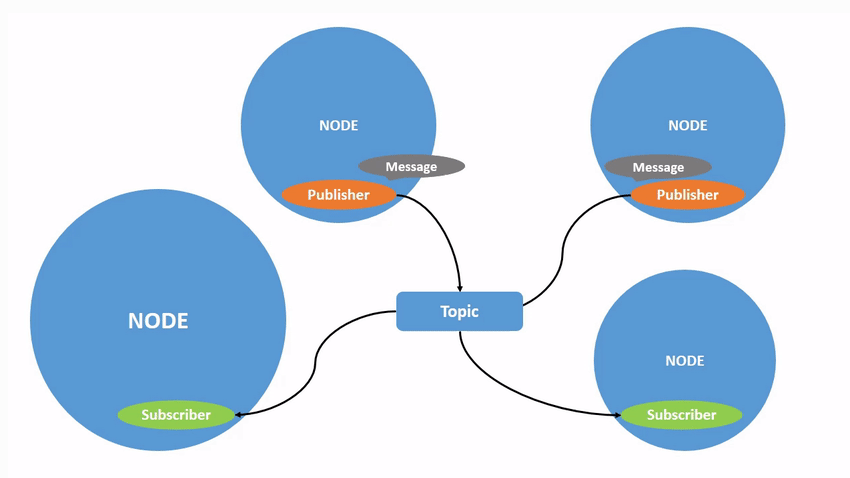
\includegraphics[width=0.7\textwidth]{nodes.png}
		\caption{Architecture de communication entre les nœuds ROS~2}
		\label{fig:nodes}
	\end{figure}
	
	\subsubsection{Catamaran}
	
	
	
	\subsubsection{USV et collecte de déchets marins}
	Le projet ATRON \cite{atron} illustre l'intérêt des USV pour la récupération autonome de déchets en milieu océanique : il motive l'objectif final du laboratoire (collecte de macro-déchets) et le besoin d'un simulateur fiable. Les auteurs y soulignent que la fiabilité de la phase de détection-collecte dépend directement de la précision du positionnement et du contrôle bas niveau du véhicule, ce qui renforce, l'importance de disposer d'un modèle dynamique correctement validé avant d'aborder les couches supérieures de perception et de planification.
	
	Les paramètres du drone sont les suivants: 
	
	\begin{table}[H]
		\centering
		\caption{Paramètres du modèle de Fossen 3-DOF}
		\label{tab:params_wamv}
		\begin{tabular}{lll}
			\toprule
			\textbf{Paramètre} & \textbf{Signification} & \textbf{Valeur} \\
			\midrule
			$m$ & masse du WAM-V & [250] kg \\
			$x_g$ & abscisse du centre de gravité (repère corps) & [0] m \\
			$I_z$ & moment d'inertie autour de l'axe $z$ & [380] kg\,m$^2$ \\
			$\ell$ (\texttt{lever\_arm}) & bras de levier des propulseurs & [1.03] m \\
			\bottomrule
		\end{tabular}
	\end{table}
	
	\begin{figure}[H]
		\centering
		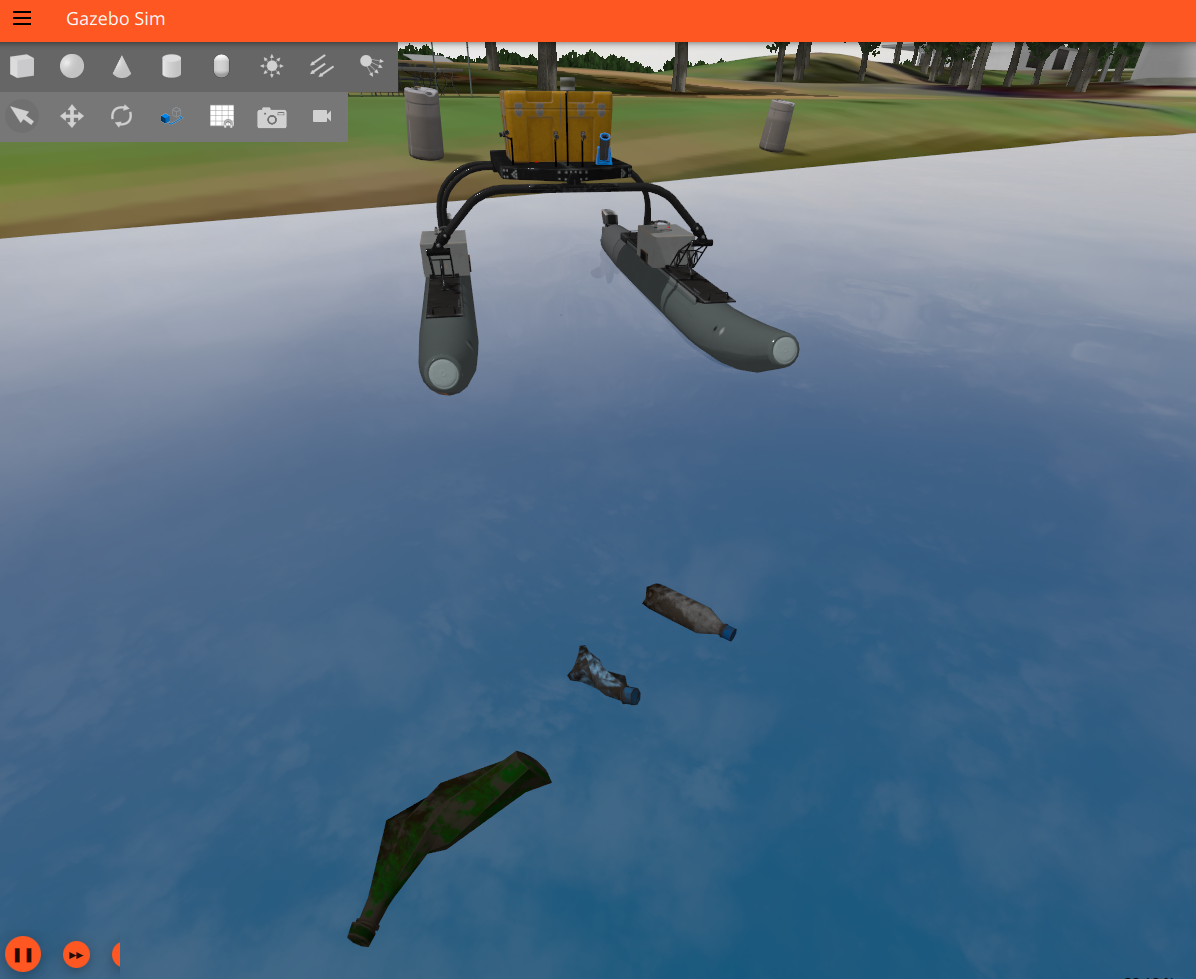
\includegraphics[width=0.9\textwidth]{garbages.png}
		\caption{Environnement VRX sous Gazebo}
		\label{fig:dechets}
	\end{figure}
	
	\begin{figure}[H]
		\centering
		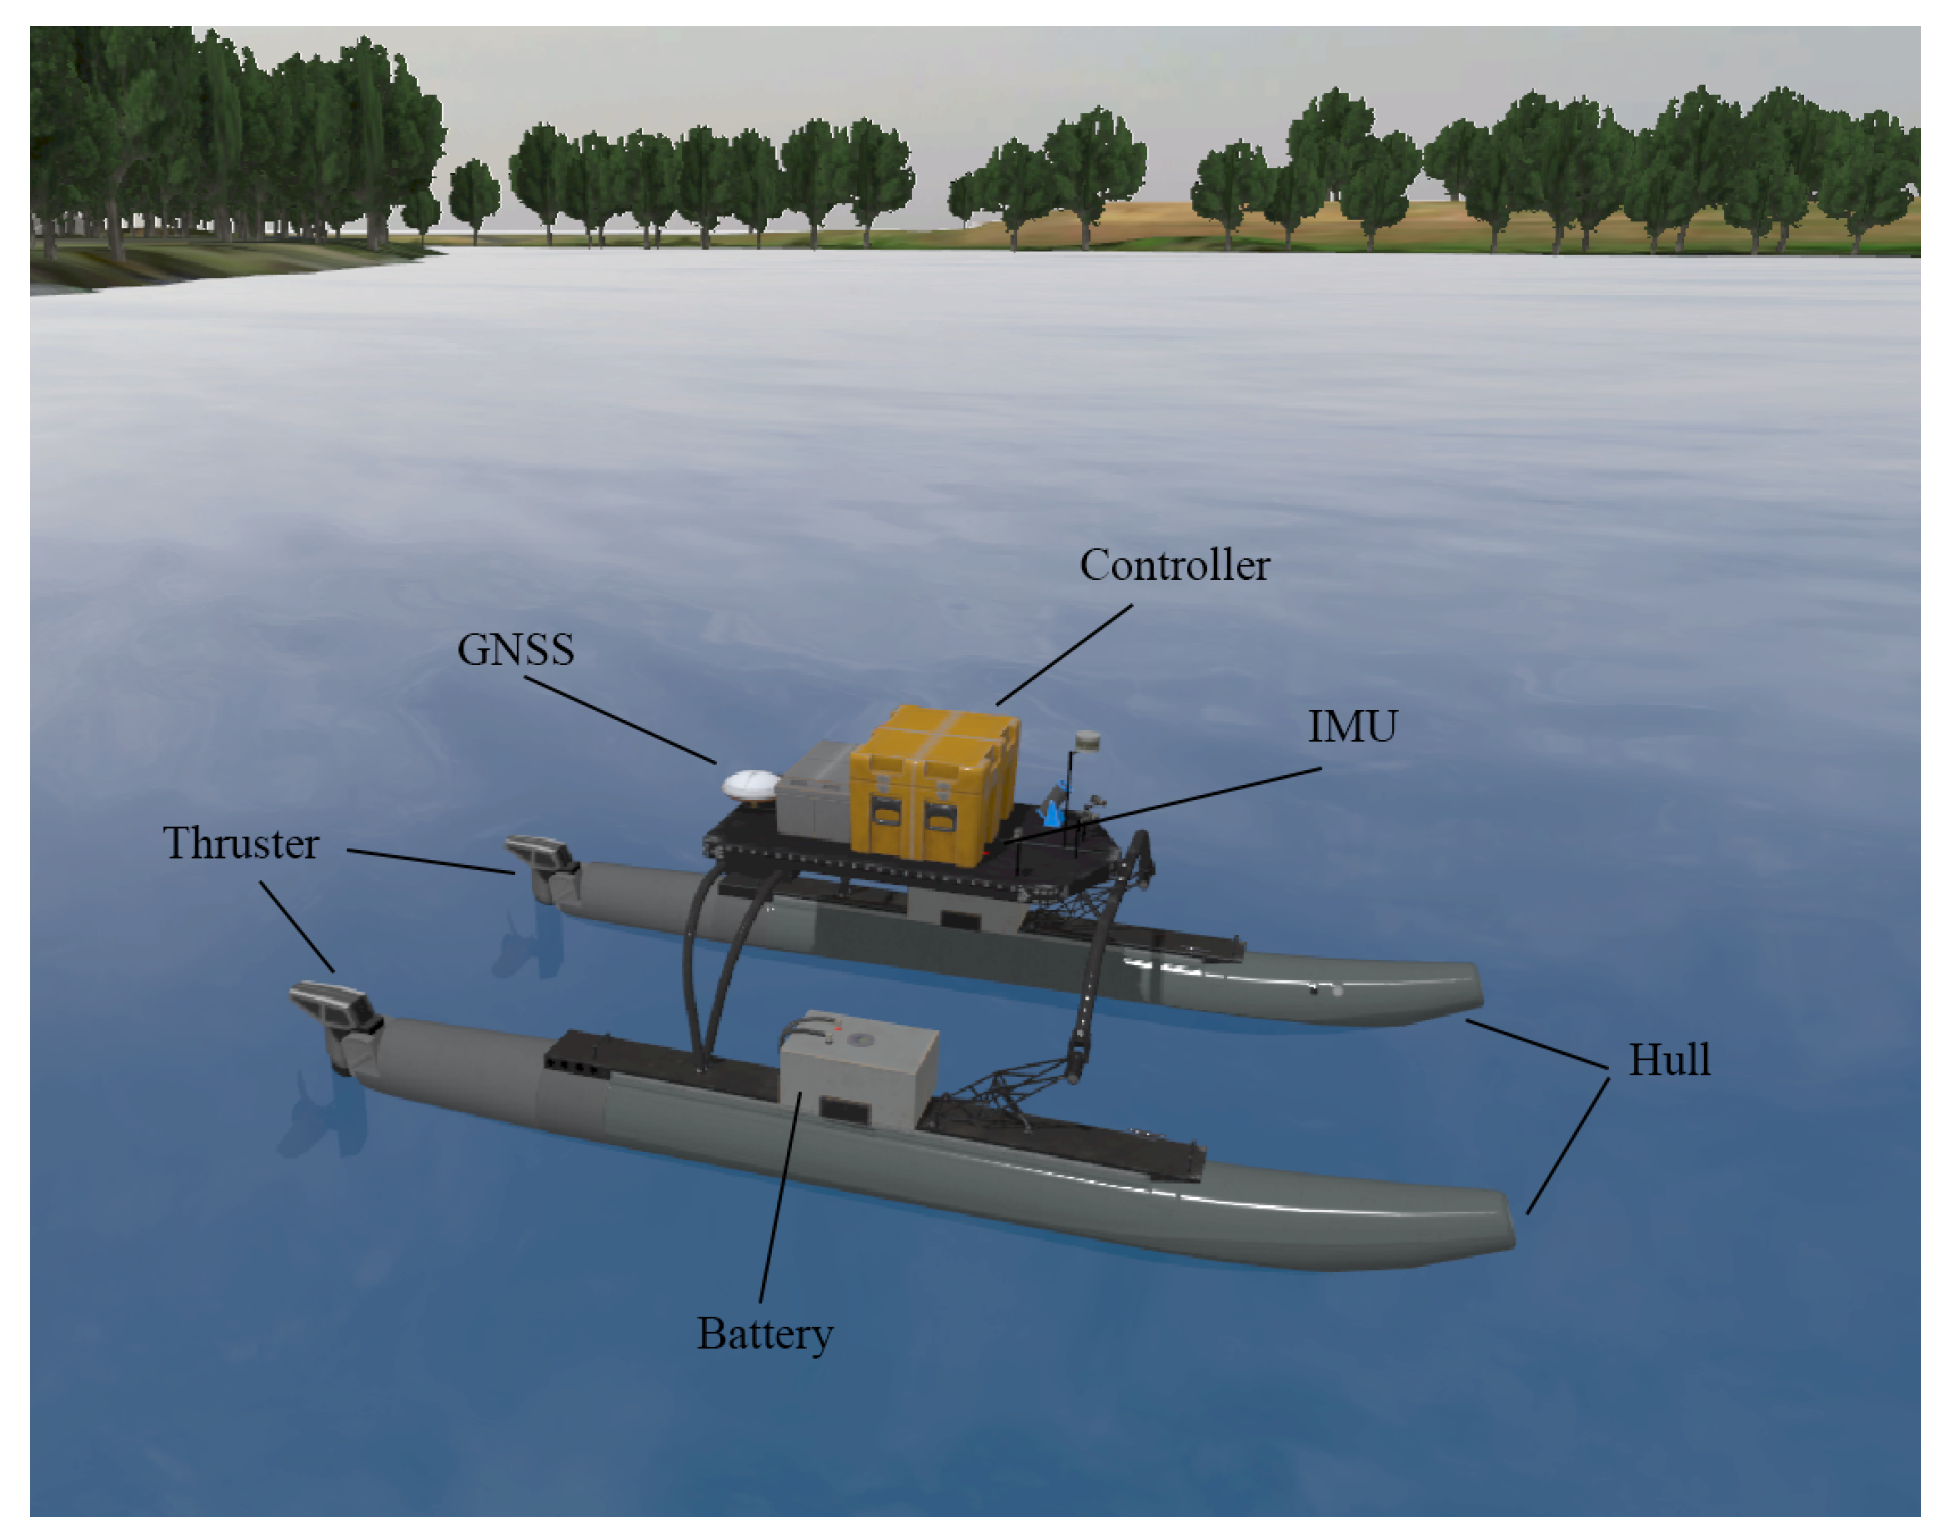
\includegraphics[width=0.9\textwidth]{parametre.png}
		\caption{Les différents composants du drone}
		\label{fig:capteurs}
	\end{figure}
	
	\subsubsection{Simulation dynamique maritime : VRX et Gazebo}
	Bingham et al. \cite{vrx} présentent le framework VRX, qui étend Gazebo à la robotique maritime (modélisation des vagues, du vent et des courants). Saldarriaga-Mesa et al. \cite{vrx2} montrent l'utilisation de VRX comme plateforme ouverte pour la conception de contrôleurs de véhicules de surface, ce qui justifie le choix de cet environnement pour notre étude. Ces deux références confirment un point méthodologique central pour notre travail : VRX repose lui-même sur une implémentation interne du modèle de Fossen pour propager la dynamique du catamaran, si bien que la \og validation\fg{} que nous menons ne compare pas la simulation à un véhicule réel, mais vérifie la cohérence entre les accélérations produites par les capteurs embarqués sur le drone et celles prédites par notre propre implémentation indépendante des équations de Fossen.
	
	\begin{figure}[H]
		\centering
		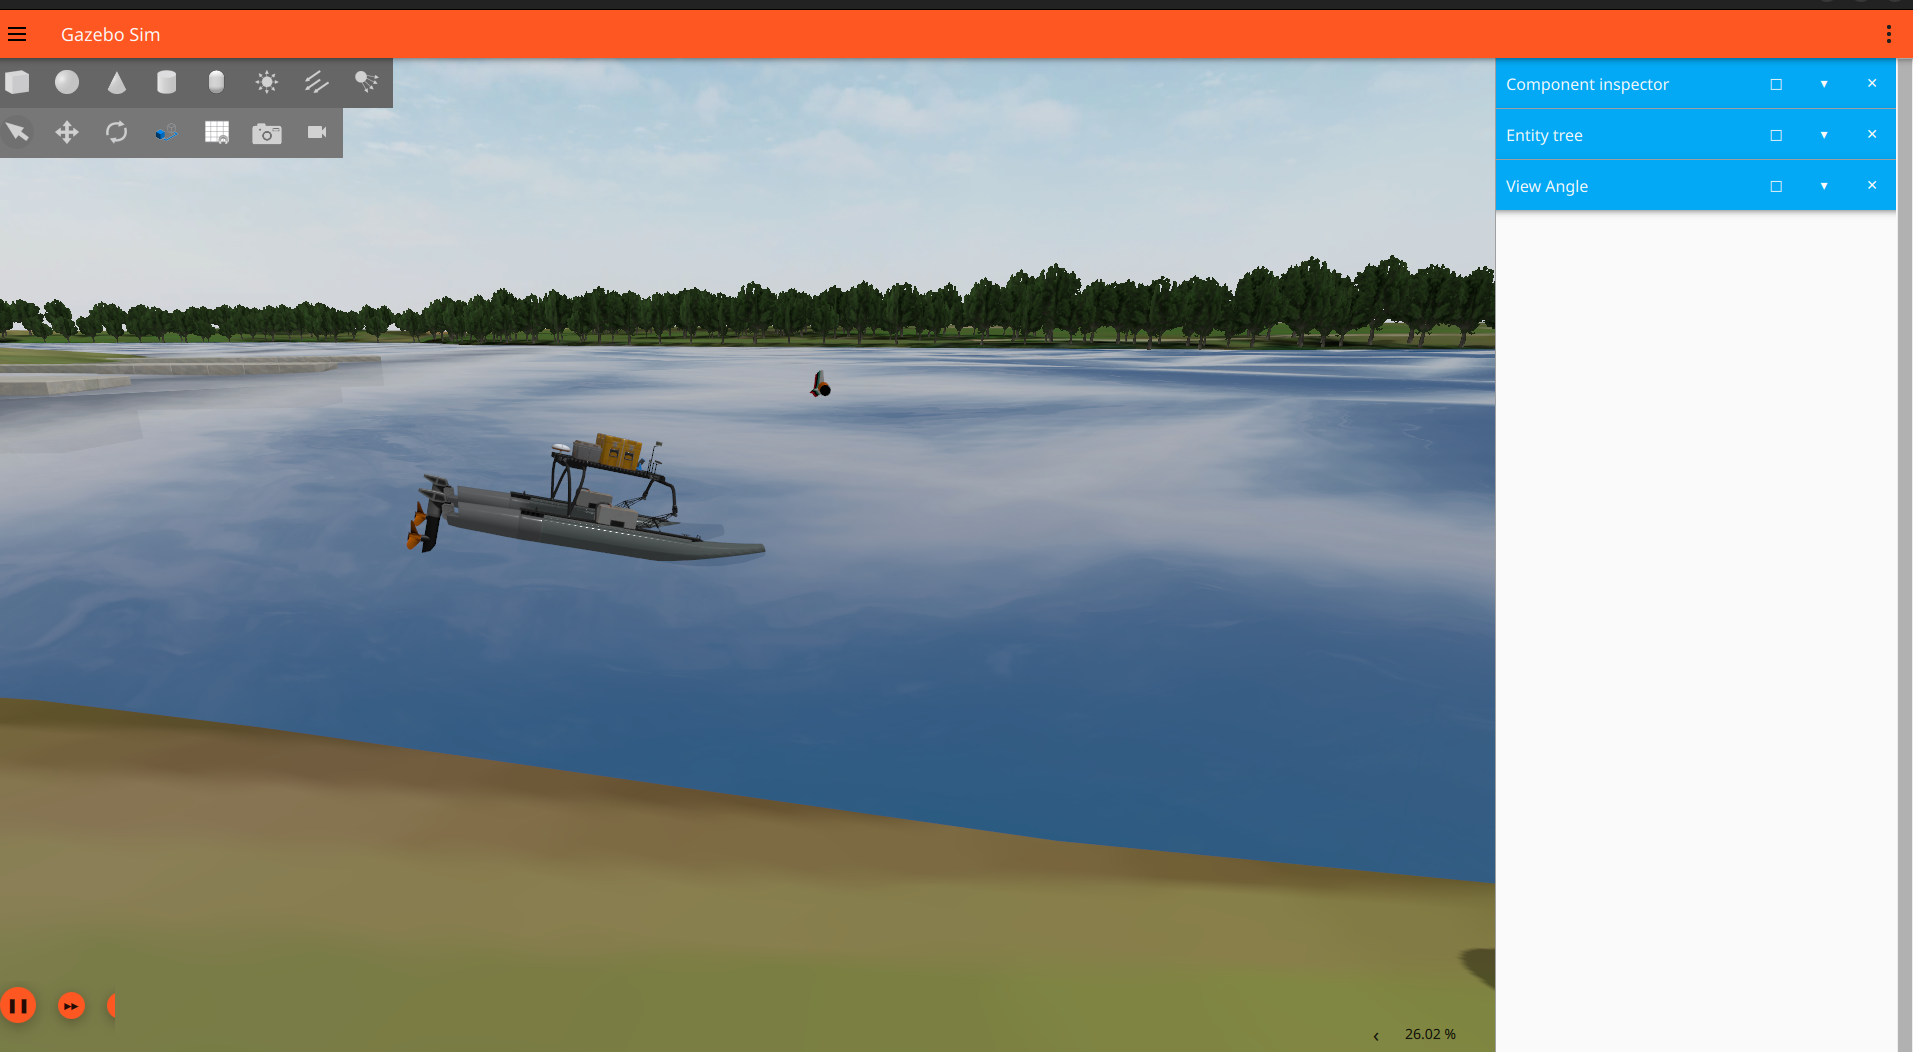
\includegraphics[width=0.9\textwidth]{wave.png}
		\caption{Environnement Sydney Regatta sous Gazebo, avec des vagues simulées permettant d'évaluer la flottabilité du drone}
		\label{fig:wave}
	\end{figure}
	
	\subsubsection{RViz2}
	
	RViz2 est un outil de visualisation intégré à l'écosystème ROS~2. Il permet de représenter graphiquement les données publiées par les différents nœuds, notamment la position du véhicule, les repères de coordonnées et les données issues des capteurs.
	
	Dans notre projet, RViz2 est principalement utilisé pour observer l'état du WAM-V et vérifier le bon fonctionnement de la chaîne de communication pendant les expérimentations et la visualisation données capteurs.
	
	\begin{figure}[H]
		\centering
		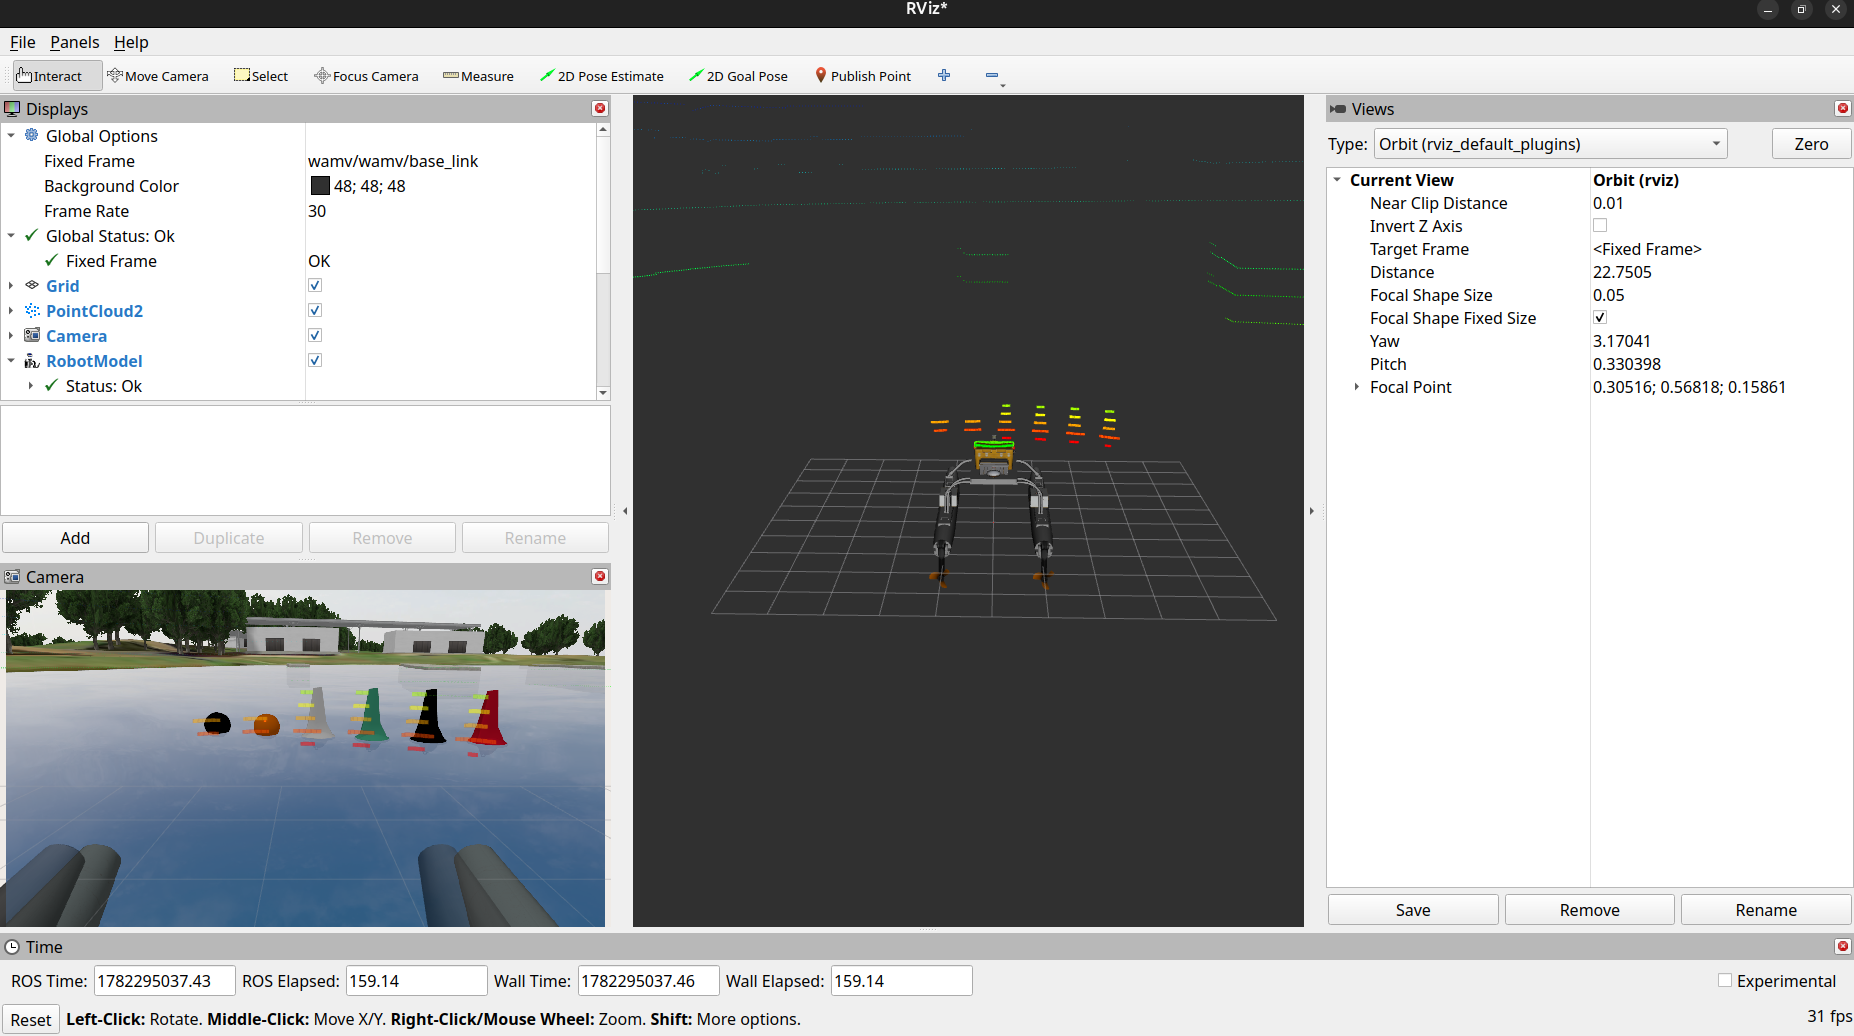
\includegraphics[width=0.7\textwidth]{Rviz2.png}
		\caption{Visualisation du système dans RViz2}
		\label{fig:rviz2}
	\end{figure}
	
	
	

\subsubsection{Modélisation des véhicules marins}

La dynamique des véhicules de surface est classiquement décrite à l'aide du formalisme de Fossen, largement utilisé pour la modélisation et l'étude des systèmes marins \cite{fossen}. Cette approche permet de représenter les différents mouvements du véhicule ainsi que les forces et moments (aérodynamiques et hydrodynamiques) qui s'exercent sur celui-ci. Elle constitue également une base de référence pour la modélisation des voiliers et autres véhicules marins autonomes \cite{lebars,saoud}.

Dans le cadre de ce travail, le drone catamaran (~\ref{fig:dechets}) est représenté par un modèle à 3 degrés de liberté, correspondant aux mouvements de translation longitudinale (\emph{surge}), de translation latérale (\emph{sway}) et de rotation autour de l'axe vertical (\emph{yaw}). Cette représentation est adaptée à un véhicule de surface dont les mouvements sont principalement considérés dans le plan horizontal. La formulation en représentation d'état permet alors de décrire l'évolution temporelle de la position, de l'orientation et des vitesses du véhicule \cite{jaulin_etat}.

Le modèle retenu prend ainsi en compte les principaux effets dynamiques nécessaires à la simulation du drone, notamment les termes liés à la masse et à l'inertie, les forces et moments hydrodynamiques ainsi que les actions générées par les propulseurs. Cette modélisation constitue la base du modèle dynamique utilisé dans l'environnement de simulations.
	

	

	
	% =====================================================
	% SECTION : REPRÉSENTATION DU MODÈLE DE FOSSEN
	% =====================================================
	\section{Représentation du modèle de Fossen: Pour un catamaran}
	\label{sec:fossen}
	
	Le comportement dynamique du drone est décrit par le formalisme matriciel de Fossen, aujourd'hui
	devenu la référence pour la modélisation et la commande des véhicules marins. Cette section en
	rappelle la construction, depuis la formulation générale à six degrés de liberté jusqu'à la
	réduction à trois degrés utilisée dans notre travail.
	
	L'approche de Fossen est devenue un modèle fondamental en hydrodynamique marine et en
	contrôle du mouvement, largement adopté dans la recherche académique et les applications
	industrielles.
	
	Cette représentation matricielle est particulièrement précieuse pour la conception des systèmes de
	guidage, de navigation et de contrôle
	
	\subsection{Formulation générale en six degrés de liberté}
	
	\subsubsection{Équations du mouvement}
	
	Les équations du mouvement d'un véhicule marin à six degrés de liberté s'écrivent, dans le repère
	corps, sous la forme matricielle compacte :
	\begin{equation}
		\boldsymbol{M}\,\dot{\boldsymbol{\nu}} + \boldsymbol{C}(\boldsymbol{\nu})\,\boldsymbol{\nu}
		+ \boldsymbol{D}(\boldsymbol{\nu})\,\boldsymbol{\nu} + \boldsymbol{g}(\boldsymbol{\eta})
		= \boldsymbol{\tau}
		\label{eq:fossen6dof}
	\end{equation}
	associée à l'équation cinématique :
	\begin{equation}
		\dot{\boldsymbol{\eta}} = \boldsymbol{J}(\boldsymbol{\eta})\,\boldsymbol{\nu}
		\label{eq:cinematique}
	\end{equation}
	
	Les variables mises en jeu suivent la terminologie standard de la \emph{Society of Naval Architects
		and Marine Engineers} (SNAME) \cite{sname}, résumée dans le tableau~\ref{tab:sname}.
	
	\begin{table}[H]
		\centering
		\caption{Notation SNAME des variables dynamiques d'un véhicule marin}
		\label{tab:sname}
		\begin{tabular}{ccccc}
			\toprule
			\textbf{Axe} & \textbf{Position} & \textbf{Angle} & \textbf{Vitesse linéaire}
			& \textbf{Vitesse angulaire} \\
			\midrule
			$X$ & $x$ & $\phi$ (roulis) & $u$ & $p$ \\
			$Y$ & $y$ & $\theta$ (tangage) & $v$ & $q$ \\
			$Z$ & $z$ & $\psi$ (lacet) & $w$ & $r$ \\
			\bottomrule
		\end{tabular}
	\end{table}
	
	Dans les équations~\eqref{eq:fossen6dof}--\eqref{eq:cinematique}, les vecteurs sont :
	\begin{itemize}[label=--]
		\item $\boldsymbol{\eta} = [x, y, z, \phi, \theta, \psi]^\top$ : position et orientation dans le
		repère Nord-Est-Bas (NED) ;
		\item $\boldsymbol{\nu} = [u, v, w, p, q, r]^\top$ : vitesses linéaires et angulaires dans le
		repère corps (BODY) ;
		\item $\boldsymbol{\tau}$ : couple des forces généralisées (propulsion, vent, houle, courants).
	\end{itemize}
	
	Les matrices de l'équation~\eqref{eq:fossen6dof} représentent :
	\begin{itemize}[label=--]
		\item $\boldsymbol{M}$ : matrice d'inertie, combinant les effets de corps rigide et de masse
		ajoutée ;
		\item $\boldsymbol{C}(\boldsymbol{\nu})$ : matrice de Coriolis et centrifuge (corps rigide et
		masse ajoutée) ;
		\item $\boldsymbol{D}(\boldsymbol{\nu})$ : matrice d'amortissement hydrodynamique ;
		\item $\boldsymbol{g}(\boldsymbol{\eta})$ : forces et moments hydrostatiques (gravité et
		flottabilité) ;
		\item $\boldsymbol{J}(\boldsymbol{\eta})$ : matrice de transformation entre les repères BODY et NED.
	\end{itemize}
	
	\subsubsection{Cinématique}
	
	L'équation cinématique~\eqref{eq} utilise les angles d'Euler pour décrire la transformation entre le repère lié au véhicule et un repère de navigation fixe, défini localement par rapport à la Terre. Les rotations
	séquentielles s'effectuent dans l'ordre lacet ($z$), tangage ($y$), roulis ($x$). La matrice de
	transformation est :
	\begin{equation}
		\boldsymbol{J}(\boldsymbol{\eta}) =
		\begin{bmatrix}
			\boldsymbol{R}(\boldsymbol{\Theta}) & \boldsymbol{0}_{3\times3} \\
			\boldsymbol{0}_{3\times3} & \boldsymbol{T}(\boldsymbol{\Theta})
		\end{bmatrix}
		\label{eq:J}
	\end{equation}
	où $\boldsymbol{R}(\boldsymbol{\Theta})$ est la matrice de rotation des vitesses de translation et
	$\boldsymbol{T}(\boldsymbol{\Theta})$ la matrice de transformation des vitesses angulaires, avec
	$\boldsymbol{\Theta} = [\phi, \theta, \psi]^\top$. Pour le drone, dont les mouvements de roulis et de
	tangage restent faibles en régime de navigation nominal, cette transformation se réduit en pratique à
	une simple rotation planaire d'angle $\psi$ entre repère corps et repère fixe, ce qui justifie a
	posteriori la réduction au modèle 3-DOF présentée en section~\ref{sec:3dof}.
	
	\subsection{Paramètres hydrodynamiques du modèle}
	\label{sec:parametres}
	
	Le tableau~\ref{tab:params} liste les paramètres du modèle 3-DOF. Ces coefficients (masse, position du centre de gravité, moment
	d'inertie) provient directement de la description URDF/SDF (ce sont des fichiers permettent de décrire la structure et les propriétés physiques du véhicule, ses liens, articulations, capteurs et l'ajustement des coefficients aerodynamiques et hydrodynamiques de l'environement) du catamaran et du fichier de description de l'environement sydney regatta.
	
	\begin{table}[H]
		\centering
		\caption{Paramètres du modèle de Fossen 3-DOF}
		\label{tab:params}
		\begin{tabular}{lll}
			\toprule
			\textbf{Paramètre} & \textbf{Signification} & \textbf{Valeur} \\
			\midrule
			$X_{\dot u}, Y_{\dot v}, Y_{\dot r}, N_{\dot v}, N_{\dot r}$ & masses ajoutées & [-100, -80, - 60, 0, 0] \\
			$X_u, X_{uu}$ & amortissement linéaire/quadratique en surge & [-50, -180] \\
			$Y_v, Y_{vv}$ & amortissement linéaire/quadratique en sway & [-80, -200] \\
			$N_r, N_{rr}$ & amortissement linéaire/quadratique en yaw & [-100 ,-300] \\
			$k$ (\texttt{thrust\_scale}) & conversion consigne $\rightarrow$ poussée & [1] N/unité \\
			\bottomrule
		\end{tabular}
	\end{table}
	
\subsubsection{Cinétique}

La cinétique décrit comment le véhicule réagit lorsqu'il se déplace ou change de direction. Elle prend notamment en compte sa masse, son inertie ainsi que les effets de l'eau sur son mouvement.

La masse totale du véhicule est composée de sa masse propre et d'une masse supplémentaire liée à l'eau déplacée pendant le mouvement. De même, les effets liés aux changements de mouvement prennent en compte à la fois le comportement du véhicule et celui de l'eau :

\begin{equation} \boldsymbol{M} = \boldsymbol{M}_{RB} + \boldsymbol{M}_{A}, \qquad \boldsymbol{C}(\boldsymbol{\nu}) = \boldsymbol{C}_{RB}(\boldsymbol{\nu}) + \boldsymbol{C}_{A}(\boldsymbol{\nu}) 
\end{equation}

où $\boldsymbol{M}_{RB}$ représente les propriétés physiques du véhicule (masse et inertie), tandis que $\boldsymbol{M}_{A}$ représente l'effet de l'eau sur son mouvement, appelé \textit{masse ajoutée}. Les termes $\boldsymbol{C}_{RB}$ et $\boldsymbol{C}_{A}$ représentent les effets liés aux changements de mouvement du véhicule et de l'eau \cite{bingham19toward,fossen}.

Enfin, le mouvement du véhicule est également ralenti par les forces de résistance de l'eau. Ces forces augmentent généralement avec la vitesse et peuvent être modélisées par :

\begin{equation} \boldsymbol{D}(\boldsymbol{\nu}) = \boldsymbol{D}_L + \boldsymbol{D}_{NL}|\boldsymbol{\nu}| \end{equation}

où $\boldsymbol{D}_{L}$ représente les résistances qui varient de manière approximativement proportionnelle à la vitesse, tandis que $\boldsymbol{D}_{NL}$ représente les résistances qui augmentent plus fortement lorsque la vitesse augmente.

	
	
	\subsection{Équations du mouvement et forces environnementales}
	
	Les forces environnementales sont intégrées à l'aide de la vitesse relative pour les courants
	océaniques, tandis que les efforts de vent et des vagues sont ajoutés par superposition linéaire. La
	vitesse relative $\boldsymbol{\nu}_r$ tient compte de l'influence d'un courant océanique irrotationnel
	de vitesse $\boldsymbol{\nu}_c$ : l'interaction du véhicule avec le fluide environnant dépend en effet
	de la vitesse relative par rapport à l'eau. Le modèle devient :
	\begin{equation}
		\boldsymbol{M}\,\dot{\boldsymbol{\nu}} + \boldsymbol{C}(\boldsymbol{\nu})\,\boldsymbol{\nu}
		+ \boldsymbol{D}(\boldsymbol{\nu})\,\boldsymbol{\nu} + \boldsymbol{g}(\boldsymbol{\eta})
		= \boldsymbol{\tau}_{prop} + \boldsymbol{\tau}_{vent} + \boldsymbol{\tau}_{vagues}
		\label{eq:relatif}
	\end{equation}
	où le torseur total se décompose en :
	\begin{itemize}[label=--]
		\item $\boldsymbol{\tau}_{prop}$ : forces de propulsion ;
		\item $\boldsymbol{\tau}_{vent}$ : forces aérodynamiques dues au vent ;
		\item $\boldsymbol{\tau}_{vague}$ : forces induites par les vagues.
	\end{itemize}
	
	Dans le cadre de nos campagnes d'expériences, le monde \texttt{sydney\_regatta} n'imposait pas de courant marin actif ; le terme
	$\boldsymbol{\nu}_c$ a donc été fixé à zéro, mais l'implémentation conserve
	l'architecture nécessaire à son activation future, ce qui facilitera l'extension du protocole à des
	scénarios avec courant.
	
\subsection{Réduction au cas 3-DOF d'un véhicule de surface}
\label{sec:3dof}

Le modèle général de Fossen décrit les six degrés de liberté d'un véhicule marin :
\emph{surge}, \emph{sway}, \emph{heave}, \emph{roll}, \emph{pitch} et \emph{yaw}.
Dans le cas d'un véhicule de surface évoluant principalement dans le plan horizontal, ce modèle peut être réduit à trois degrés de liberté.

Cette réduction repose sur les hypothèses suivantes :
\begin{itemize}
	\item \textbf{H1 :} le véhicule reste à la surface de l'eau, sa position verticale est supposée constante et les mouvements de \emph{heave} sont donc négligés ;
	\item \textbf{H2 :} les mouvements de \emph{roll} (roulis) et de \emph{pitch} (tangage) sont supposés faibles devant les mouvements horizontaux et sont donc négligés ;
	\item \textbf{H3 :} les effets de couplage liés aux mouvements négligés sont supposés suffisamment faibles pour être ignorés dans le modèle retenu.
\end{itemize}

Sous ces hypothèses, seuls les mouvements de \emph{surge}, \emph{sway} et \emph{yaw} sont conservés. Le vecteur des vitesses devient alors
\begin{equation}
	\boldsymbol{\nu} =
	[u,v,r]^\top,
\end{equation}
où $u$ représente la vitesse longitudinale, $v$ la vitesse latérale et $r$ la vitesse de rotation autour de l'axe vertical.

Les forces de rappel $\boldsymbol{g}(\boldsymbol{\eta})$, principalement associées à la gravité et à la flottabilité, ne sont pas considérées dans cette représentation car les mouvements verticaux, le roulis et le tangage sont supposés négligeables. Le modèle dynamique se réduit ainsi à :

\begin{equation}
	\boldsymbol{M}\dot{\boldsymbol{\nu}}
	+
	\boldsymbol{C}(\boldsymbol{\nu})\boldsymbol{\nu}
	+
	\boldsymbol{D}(\boldsymbol{\nu})\boldsymbol{\nu}
	=
	\boldsymbol{\tau}
	\label{eq:fossen3dof}
\end{equation}

où $\boldsymbol{M}$ représente les effets d'inertie et de masse ajoutée, $\boldsymbol{C}(\boldsymbol{\nu})$ les effets liés aux changements de mouvement, $\boldsymbol{D}(\boldsymbol{\nu})$ les forces de résistance de l'eau et $\boldsymbol{\tau}$ les forces et moments appliqués au véhicule.

Les matrices du modèle 3-DOF prennent la forme suivante :

\begin{itemize}
	\item Matrice d'inertie $\boldsymbol{M}$: elle regroupe la masse du véhicule et les effets de masse ajoutée de l'eau :
	\begin{equation}
		\boldsymbol{M} = \begin{bmatrix}
			m - X_{\dot u} & 0 & 0 \\
			0 & m - Y_{\dot v} & m x_g - Y_{\dot r} \\
			0 & m x_g - N_{\dot v} & I_z - N_{\dot r}
		\end{bmatrix}
		\label{eq:M3dof}
	\end{equation}
	
	\item Matrice de Coriolis $\boldsymbol{C}(\boldsymbol{\nu})$: elle représente les effets liés au couplage entre les différents mouvements du véhicule :
	\begin{equation}
		\boldsymbol{C}(\boldsymbol{\nu}) = \begin{bmatrix}
			0 & 0 & -(m - Y_{\dot v}),v - (m x_g - Y_{\dot r}),r \\
			0 & 0 & (m - X_{\dot u}),u \\
			(m - Y_{\dot v}),v + (m x_g - Y_{\dot r}),r & -(m - X_{\dot u}),u & 0
		\end{bmatrix}
		\label{eq:C3dof}
	\end{equation}
	
	\item Matrice d'amortissement $\boldsymbol{D}(\boldsymbol{\nu})$: elle représente les forces de résistance exercées par l'eau sur le véhicule. Les dérivées hydrodynamiques étant négatives, elle est définie par :
	\begin{equation}
		\boldsymbol{D}(\boldsymbol{\nu}) =
		-\begin{bmatrix}
			X_u + X_{uu}|u| & 0 & 0 \\
			0 & Y_v + Y_{vv}|v| & 0 \\
			0 & 0 & N_r + N_{rr}|r|
		\end{bmatrix}
		\label{eq:D3dof}
	\end{equation}
\end{itemize}


La résolution du modèle consiste alors à déterminer l'accélération du véhicule à partir des forces et moments qui lui sont appliqués :
\begin{equation}
	\dot{\boldsymbol{\nu}} =
	\boldsymbol{M}^{-1}
	\left(
	\boldsymbol{\tau}
	-
	\boldsymbol{C}(\boldsymbol{\nu}),\boldsymbol{\nu}
	-
	\boldsymbol{D}(\boldsymbol{\nu}),\boldsymbol{\nu}
	\right)
	\label{eq:nudot}
\end{equation}

	
	
	
	
	
	\subsection{Torseur de propulsion}
	
	Les deux propulseurs fixes du drone, alignés avec l'axe $x$ du repère corps et séparés par un bras de
	levier $2\ell$, produisent une poussée différentielle. Le torseur de propulsion s'écrit :
	\begin{equation}
		X_{prop} = k\,(T_L + T_R), \qquad Y_{prop} = 0, \qquad N_{prop} = k\,\ell\,(T_R - T_L)
		\label{eq:thrust}
	\end{equation}
	où $k$ (\texttt{thrust\_scale}) convertit la consigne brute en newtons et $\ell$ (\texttt{lever\_arm})
	désigne le bras de levier. La somme des poussées agit en surge, leur différence en lacet : c'est le
	principe de la poussée différentielle exploité par le programme de guidage.
	
	\subsection{Modélisation des forces de vent et de houle}
	
	\subsubsection{Forces de vent}
	
	Le vent est modélisé par une loi quadratique en vitesse relative, conformément au modèle VRX
	\cite{vrx}. En notant $V_w$ la vitesse du vent, $\beta$ sa direction et $\psi$ le cap du véhicule, on
	définit les composantes du vent dans le repère corps:
	\begin{equation}
		u_w = V_w \cos(\beta - \psi), \qquad v_w = V_w \sin(\beta - \psi)
	\end{equation}
	puis les vitesses relatives $u_{rw} = u - u_w$ et $v_{rw} = v - v_w$, qui donnent :
	\begin{equation}
		X_{vent} = c_x\,u_{rw}|u_{rw}|, \quad
		Y_{vent} = c_y\,v_{rw}|v_{rw}|, \quad
		N_{vent} = -2\,c_n\,u_{rw}\,v_{rw}
		\label{eq:vent}
	\end{equation}
	Les coefficients $c_x$, $c_y$ et $c_n$ dépendent de la surface exposée au vent du WAM-V selon chaque
	axe et sont, en toute rigueur, fonction de l'angle d'incidence relatif $\beta - \psi$ ; dans un premier
	temps, et conformément à l'implémentation par défaut de VRX, ils ont été considérés constants, ce qui
	constitue une simplification à garder à l'esprit lors de l'interprétation des écarts observés en sway.
	
	
		\begin{figure}[H]
		\centering
		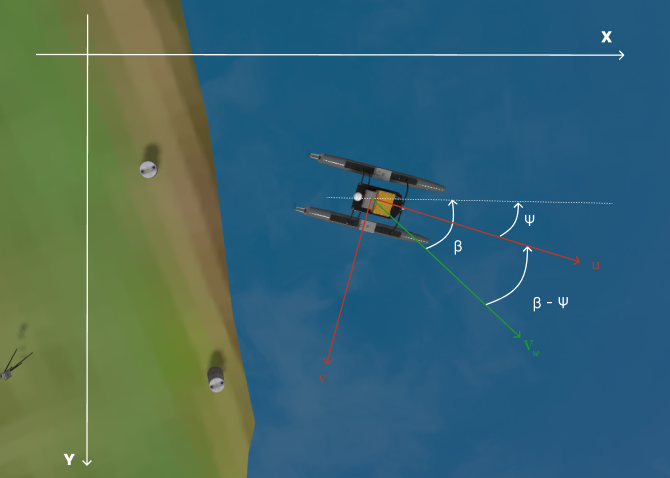
\includegraphics[width=0.7\textwidth]{repere_vent.png} 
		\caption{}
		\label{fig:vent}
	\end{figure}
	

	\subsubsection{Forces des vagues}
	
	La houle est représentée par une dérive moyenne plus une oscillation du premier ordre à la période pic
	$T_p$. Pour chaque axe ($X$, $Y$, $N$) :
	\begin{equation}
		X_{houle}(t) = X_{drift} + A_X \cos(\omega_p\,t + \varphi_X), \qquad \omega_p = \frac{2\pi}{T_p}
		\label{eq:houle}
	\end{equation}
	Cette formulation du premier ordre néglige les effets de dérive lente (second ordre) et les
	interactions non linéaires entre plusieurs composantes spectrales de la houle ; elle reste néanmoins
	cohérente avec le spectre de houle relativement étroit généré par défaut dans le monde
	\texttt{sydney\_regatta}, où une unique période pic $T_p$ domine l'excitation.
	
	

	
	\section{Validation}
	
		\subsection{Mise en place de l'environnement de simulation}
	
	\subsubsection{Chaîne logicielle}
	L'environnement repose sur Ubuntu~22.04, ROS~2 (Jazzy), Gazebo (Harmonic) et le monde \texttt{sydney\_regatta} (voir figure~\ref{fig:wave}) de VRX, qui fournit le modèle drone équipé de deux propulseurs différentiels, d'une IMU, d'une caméra RGB et d'un LiDAR 3D. RViz2 assure la visualisation des flux capteurs. Ce choix de version (Jazzy + Harmonic) correspond à la configuration officiellement supportée par le dépôt VRX au moment du stage ; il a été privilégié à des versions plus récentes de ROS~2 afin de limiter les risques d'incompatibilité avec les plugins Gazebo fournis par le projet.
	
	\subsubsection{Architecture de communication}
	Deux middlewares coexistent : le transport Gazebo (topics de simulation : pose (position à partir du GPS), IMU, commandes de propulseurs) et ROS~2 (topic d'étiquetage \verb|/usv/current_segment|). Le tableau~\ref{tab:topics} résume les flux utilisés. Cette coexistence de deux bus de communication est une contrainte structurante du projet VRX : le moteur physique (Gazebo Transport) et la couche applicative (ROS~2, via \texttt{ros\_gz\_bridge}) ne partagent pas nativement le même espace de nommage, ce qui a nécessité un pont explicite pour certains topics et une vigilance particulière sur la synchronisation temporelle des messages lors de l'enregistrement.
	
	\begin{table}[H]
		\centering
		\caption{Principaux topics de la chaîne d'acquisition}
		\label{tab:topics}
		\begin{tabular}{lll}
			\toprule
			\textbf{Topic} & \textbf{Middleware} & \textbf{Contenu} \\
			\midrule
			\verb|/world/sydney_regatta/pose/info| & Gazebo & la position dans le repère monde \\
			\verb|.../imu_wamv_sensor/imu| & Gazebo & accélérations et vitesses angulaires IMU \\
			\verb|/wamv/thrusters/left/thrust|  & Gazebo & commande propulseur gauche $T_L$ \\
			\verb|/wamv/thrusters/right/thrust| & Gazebo & commande propulseur droit $T_R$ \\
			\verb|/usv/current_segment| & ROS~2 & étiquette de l'expérience en cours \\
			\bottomrule
		\end{tabular}
	\end{table}
	
	\subsubsection{Difficultés rencontrées}
	L'installation a nécessité la résolution d'incompatibilités de dépendances (versions de paquets ROS/Gazebo, pilotes graphiques). Le parsing des messages Gazebo au format texte (protobuf) a imposé un analyseur robuste par expressions régulières.
	
	Trois catégories de difficultés méritent d'être détaillées, car elles ont représenté une part significative du temps d'ingénierie du stage :
	\begin{itemize}[label=--]
		\item \textbf{Dépendances logicielles.} Les versions de \texttt{ros\_gz}, de Gazebo Harmonic et des pilotes graphiques (OpenGL/Vulkan) doivent être strictement cohérentes ; une désynchronisation, même mineure, provoque des échecs silencieux au lancement du monde \texttt{sydney\_regatta} (absence de rendu, capteurs muets) plus difficiles à diagnostiquer qu'une erreur de compilation explicite.
		\item \textbf{Format des messages.} Certains messages Gazebo, exposés en texte protobuf plutôt qu'en binaire structuré, ont nécessité l'écriture d'un analyseur par expressions régulières suffisamment tolérant pour absorber les variations de mise en forme (espaces, ordre des champs) observées d'une version à l'autre du pont \texttt{ros\_gz\_bridge}.
		
	\end{itemize}
	
	\subsection{Protocole expérimental de validation}
	
	Valider le modèle dynamique consiste à exciter le système avec des entrées connues, puis à comparer les sorties mesurées aux sorties prédites par le modèle soumis aux mêmes entrées. Nous avons donc conçu un séquenceur d'expériences qui permet de téléopérer le drone par des entrées en boucle ouverte afin de collecter l'ensemble des données capteurs sur ces trajectoires parcourues.. Ce principe d'identification par excitation contrôlée est classique en automatique : il garantit que les grandeurs d'intérêt (surge, sway, yaw et leurs dérivées) sont suffisamment sollicitées sur toute la plage de fonctionnement du véhicule, condition nécessaire pour qu'une comparaison modèle/mesure soit réellement discriminante et ne se limite pas à un régime de fonctionnement particulier.
	
	
	Le tableau~\ref{tab:exp} présente les huit simulations retenues.
	
	\begin{figure}[H]
		\centering
		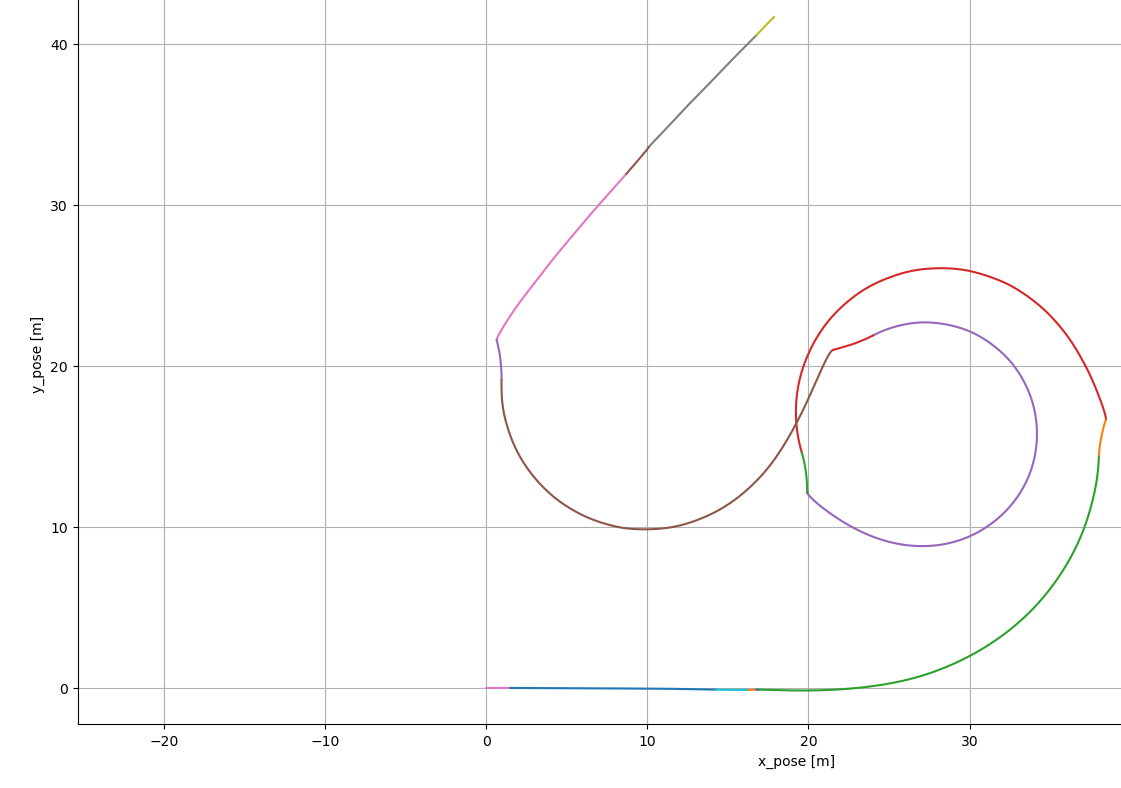
\includegraphics[width=0.7\textwidth]{traj_1.png} 
		\caption{Trajectoire suivie par le drone pour exciter sa dynamique et valider le modèle}
		\label{fig:trajectoire}
	\end{figure}
	
	\begin{table}[H]
		\centering
		\caption{Protocole d'expériences excitatrices}
		\label{tab:exp}
		\begin{tabular}{lcccl}
			\toprule
			\textbf{Expérience} & $T_L$ & $T_R$ & \textbf{Durée}  \\
			\midrule
			1 -- Accélération ligne droite & 500 & 500 & 27 s  \\
			2 -- Roue libre & 0 & 0 & 12 s & amortissement naturel \\
			3 -- Virage grand rayon & 500 & 625 & 45 s  \\
			4 -- Virage rayon moyen & 500 & 750 & 45 s \\
			5 -- Virage petit rayon & 500 & 875 & 45 s\\
			6 -- Virage opposé & 750 & 500 & 45 s  \\
			7 -- Ligne droite rapide & 625 & 625 & 20 s  \\
			8 -- Ligne droite lente & 375 & 375 & 20 s \\
			\bottomrule
		\end{tabular}
	\end{table}
	
	Le choix des couples $(T_L, T_R)$ n'est pas arbitraire : il répond à une logique d'identification progressive. Les expériences~1, 7 et~8 forment une famille de lignes droites à trois amplitudes différentes (nominale, rapide, lente), ce qui permet de vérifier que les termes d'amortissement quadratique $X_{uu}$ (tableau~\ref{sec:parametres}) de l'équation~\eqref{eq:D3dof} sont correctement identifiés sur toute la plage de vitesse, et pas seulement au point de fonctionnement nominal. Les expériences~3 à~5 font croître progressivement l'écart $T_R - T_L$ à poussée moyenne $T_L$ constante, ce qui isole l'effet du terme de lacet $N_{prop}$ (tableau~\ref{sec:parametres}) de l'équation~\eqref{eq:thrust} sans modifier simultanément l'excitation en surge. Enfin, l'expérience~6 inverse le déséquilibre de l'expérience~4 : en toute rigueur, un drone parfaitement symétrique devrait produire des trajectoires en miroir, si bien qu'un écart significatif entre ces deux expériences est un indicateur direct d'asymétrie résiduelle du modèle ou du véhicule simulé (décentrage du centre de gravité $x_g$, dissymétrie des propulseurs).
	
	
	\subsection{Grandeurs enregistrées et estimation des vitesses}
	
	L'enregistreur regroupe plusieurs flux asynchrones au sein d'un même enregistrement : la pose du drone (position, quaternion d'attitude et cap), les vitesses et accélérations dans le repère corps, les mesures brutes de l'IMU, les commandes des propulseurs ainsi que l'étiquette de l'expérience. Les vitesses linéaires dans le repère monde sont obtenues par différenciation de la pose, puis projetées dans le repère corps à l'aide du quaternion d'attitude. Les vitesses angulaires sont quant à elles déterminées à partir de la variation du quaternion. Les accélérations sont ensuite obtenues à partir de la variation des vitesses.
	
	\subsection{Validation n°1}
	\label{sec:exp_2}
	Pour chaque instant de l'enregistrement, le couple total $\tau = \tau_{prop} + \tau_{vent} + \tau_{vague}$ est reconstruit, puis calcule l'accélération $\dot\nu = M^{-1}(\tau - C\nu - D\nu)$. Trois courbes sont superposées par axe (surge, sway, yaw) : mesure IMU, dérivée cinématique et résultat de Fossen.
	
	
	La lecture visuelle des courbes est complétée par
	quatre indicateurs, l'erreur $e_i = y^{\mathrm{mes}}_i -
	y^{\mathrm{exp}}_i$ où $y^{\mathrm{mes}}$ est le signal mesuré et $y^{\mathrm{exp}}$ est le signal prédit:
	
	\begin{equation}
		\mathrm{RMSE} = \sqrt{\frac{1}{N}\sum_{i=1}^{N} e_i^{2}}
		\label{eq:rmse}
	\end{equation}
	
	\begin{equation}
		\mathrm{MAE} = \frac{1}{N}\sum_{i=1}^{N} |e_i|
		\label{eq:mae}
	\end{equation}
	
	L'objectif est de tester le modèle dans un environement calme
	\begin{table}[H]
		\centering
		\caption{Expérience 1}
		\label{tab:params_exp_2}
		\begin{tabular}{ll}
			\toprule
			\textbf{Groupe} & \textbf{Valeurs} \\
			\midrule
			Inertie & $m = 250$~kg, $I_z = 380$~kg·m², $x_g = 0$ \\
			Masse ajoutée & $X_{\dot u} = -100$, $Y_{\dot v} = -80$, $N_{\dot r} = -60$ \\
			Amortissement & $X_u = -50$, $X_{uu} = -180$, $Y_v = -80$, $Y_{vv} = -200$,
			$N_r = -100$, $N_{rr} = -300$ \\
			Propulsion & $k = 1,03$ ; $\ell = 1,0$~m \\
			Vent / vagues & \textbf{désactivés} ($V_w = 0$, amplitudes de houle nulles) \\
			\bottomrule
		\end{tabular}
	\end{table}
	
	\paragraph{Indicateurs globaux.}
	Rappel méthodologique : le modèle est évalué instantanément à partir des états mesurés
	$(u, v, r)$, sans intégration temporelle ; les courbes du modèle sont donc des restitutions
	instantanées des accélérations, comparées aux mesures IMU et cinématiques sur
	$N = 8739$ échantillons (tableau~\ref{tab:stats_exp_2}, figure~\ref{fig:exp_2}).
	
	\begin{table}[H]
		\centering
		\caption{Expérience 1 -- statistiques de l'écart modèle/mesures}
		\label{tab:stats_exp_2}
		\begin{tabular}{lcccccc}
			\toprule
			\textbf{Comparaison} & \textbf{Biais} & \textbf{Écart-type} & \textbf{RMSE}
			& \textbf{MAE} & \textbf{MaxAbsError}\\
			\midrule
			
			
			
			$\dot r$ : Fossen $-$ cinématique
			& $0,112$ & $0,277$ & $0,299$ & $0,223$
			& $0,964$  \\
			
			$a_x$ : Fossen $-$ IMU
			& $0,930$ & $1,802$ & $2,028$ & $1,035$
			& $5,923$  \\
			
			$a_y$ : Fossen $-$ IMU
			& $0,106$ & $0,229$ & $0,253$ & $0,193$
			& $0,780$  \\
			
			\bottomrule
		\end{tabular}
	\end{table}
	
	
	\begin{figure}[H]
		\centering
		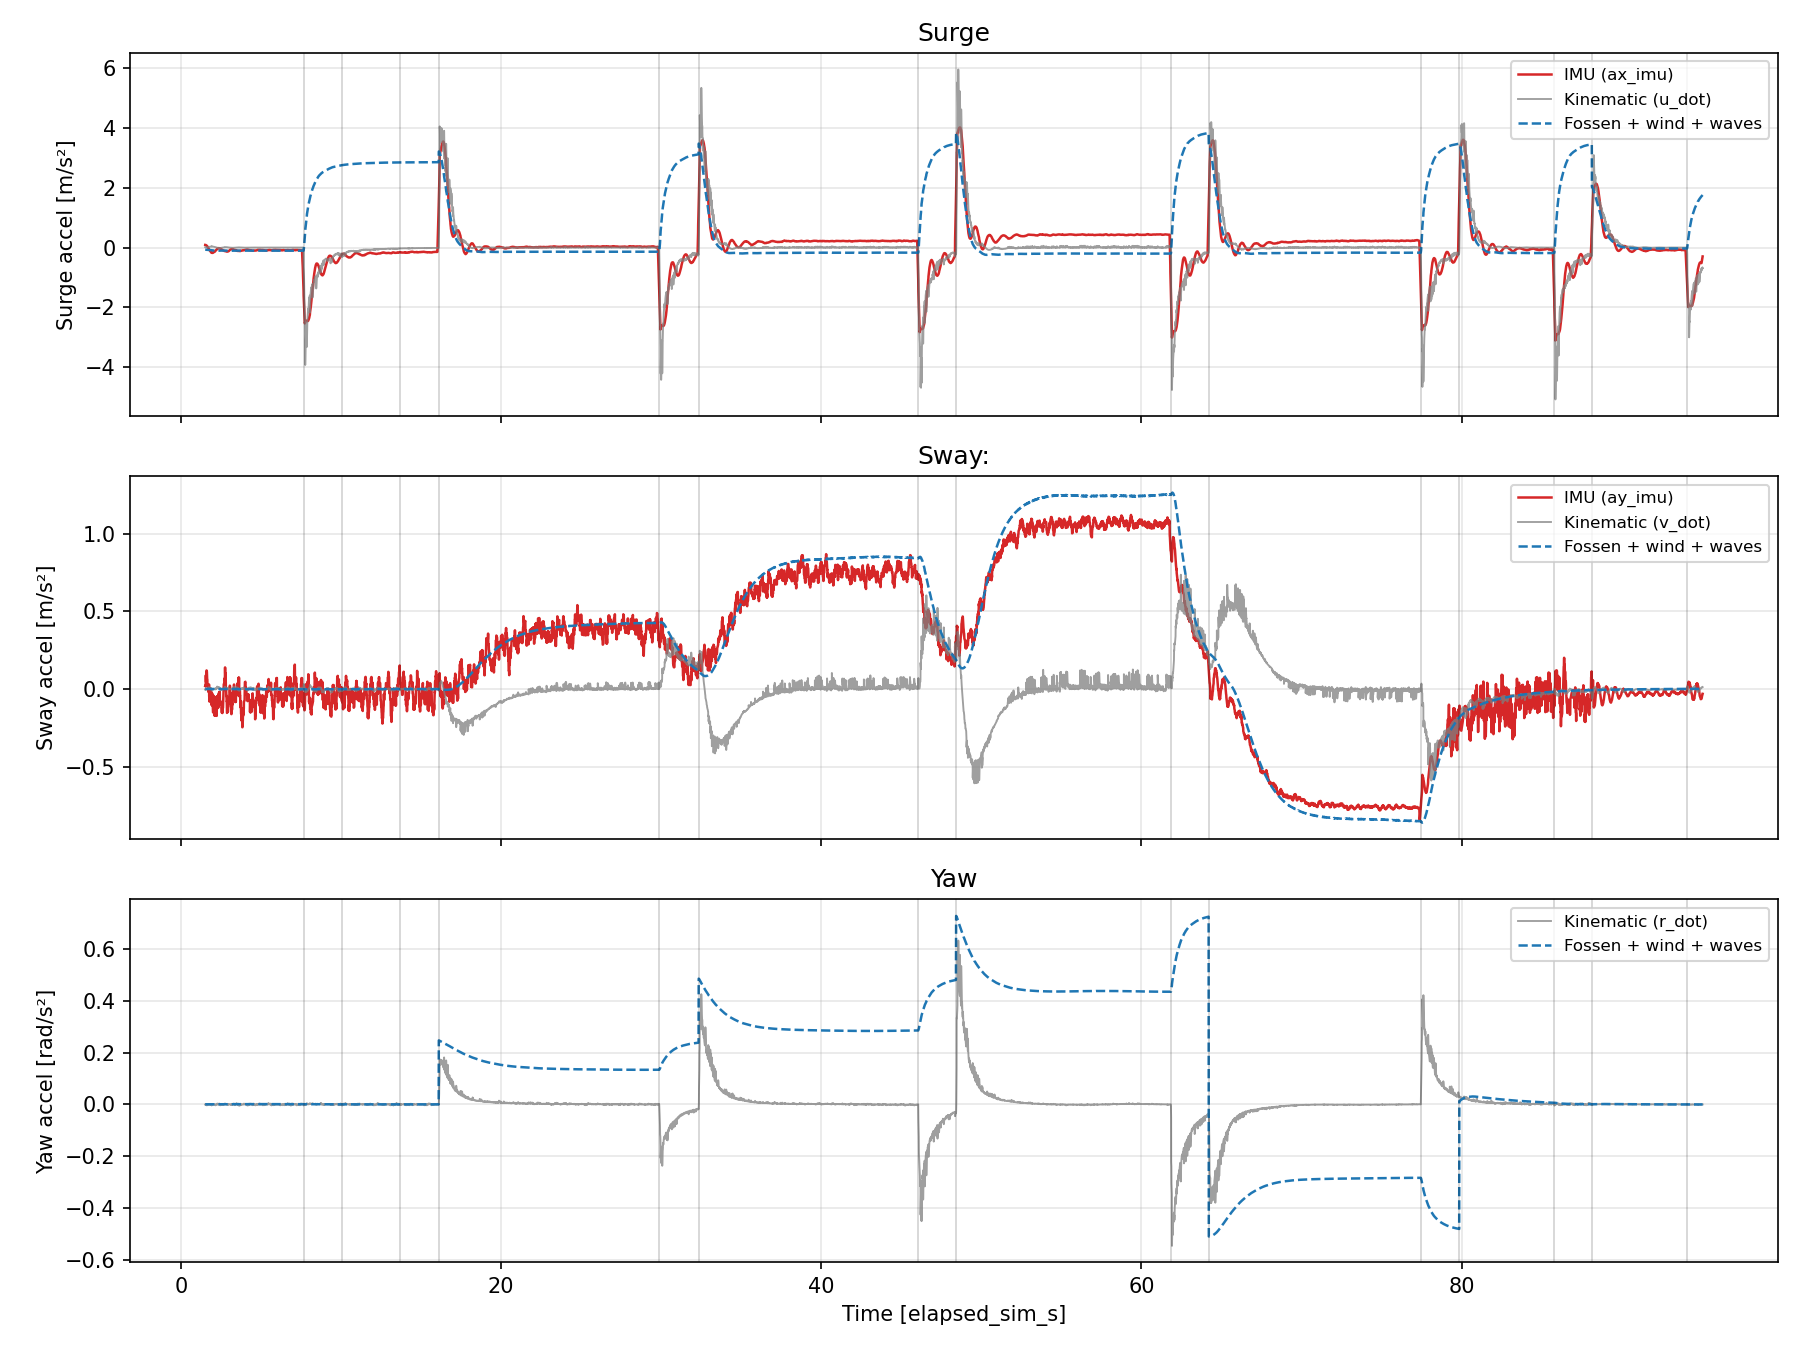
\includegraphics[width=\textwidth]{comparison_essai2.png}
		\caption{Expérience 1 -- accélérations mesurées (IMU, cinématique) et sorties du modèle de Fossen
			(vent et vagues désactivés).}
		\label{fig:exp_2}
	\end{figure}
	
	L’expérience n°1, réalisée sans vent ni houle, permet d’isoler la dynamique hydrodynamique du VRX et confirme globalement la structure du modèle de Fossen en 3~DOF. L’accord est particulièrement bon en sway (RMSE $=0{,}253$~m/s²), où le modèle reproduit les différents niveaux d’accélération et leur inversion de signe, confirmant la pertinence du terme de Coriolis $(m-X_{\dot u})ur$. En revanche, des écarts persistent en surge (RMSE $=2{,}028$~m/s²), principalement lors des changements de consigne, ainsi qu’en yaw (RMSE $=0{,}299$~rad/s²), où le modèle surestime l’accélération après le pic initial, suggérant une sous-estimation de l’amortissement hydrodynamique ($N_r,N_{rr}$). Ces résultats montrent ainsi que la formulation théorique est cohérente avec la dynamique du VRX, mais que sa précision quantitative reste limitée par les simplifications du modèle 3~DOF et les imperfections résiduelles de la simulation et des mesures.
	
	\subsection{Validation 2}
	\label{sec:exp_1}
	
	
	

	Le jeu de paramètres initial (tableau~\ref{tab:params_exp_1}) reprend des valeurs
	hydrodynamiques raisonnables pour le drone, avec $k = 1$ et $\ell = 1$~m : les consignes de
	propulsion y sont donc interprétées directement comme des newtons et des newtons-mètres.
	
	\begin{table}[H]
		\centering
		\caption{Expérience 2 -- jeu de paramètres initial}
		\label{tab:params_exp_1}
		\begin{tabular}{ll}
			\toprule
			\textbf{Groupe} & \textbf{Valeurs} \\
			\midrule
			Inertie & $m = 250$~kg, $I_z = 380$~kg·m², $x_g = 0$ \\
			Masse ajoutée & $X_{\dot u} = -100$, $Y_{\dot v} = -80$, $N_{\dot r} = -60$ \\
			Amortissement & $X_u = -50$, $X_{uu} = -180$, $Y_v = -80$, $Y_{vv} = -200$,
			$N_r = -100$, $N_{rr} = -300$ \\
			Propulsion & $k = 1,03$ ; $\ell = 1,0$~m \\
			Vent & $V_w = 5$~m/s, direction $20^\circ$, $(c_x, c_y, c_n) = (0,5;\,0,5;\,0,33)$ \\
			Houle & $T_p = 10$~s, dérive $X = 20$~N, amplitudes $60/60/30$, phases $0$\footnotemark \\
			\bottomrule
		\end{tabular}
	\end{table}

	
	\begin{figure}[H]
		\centering
		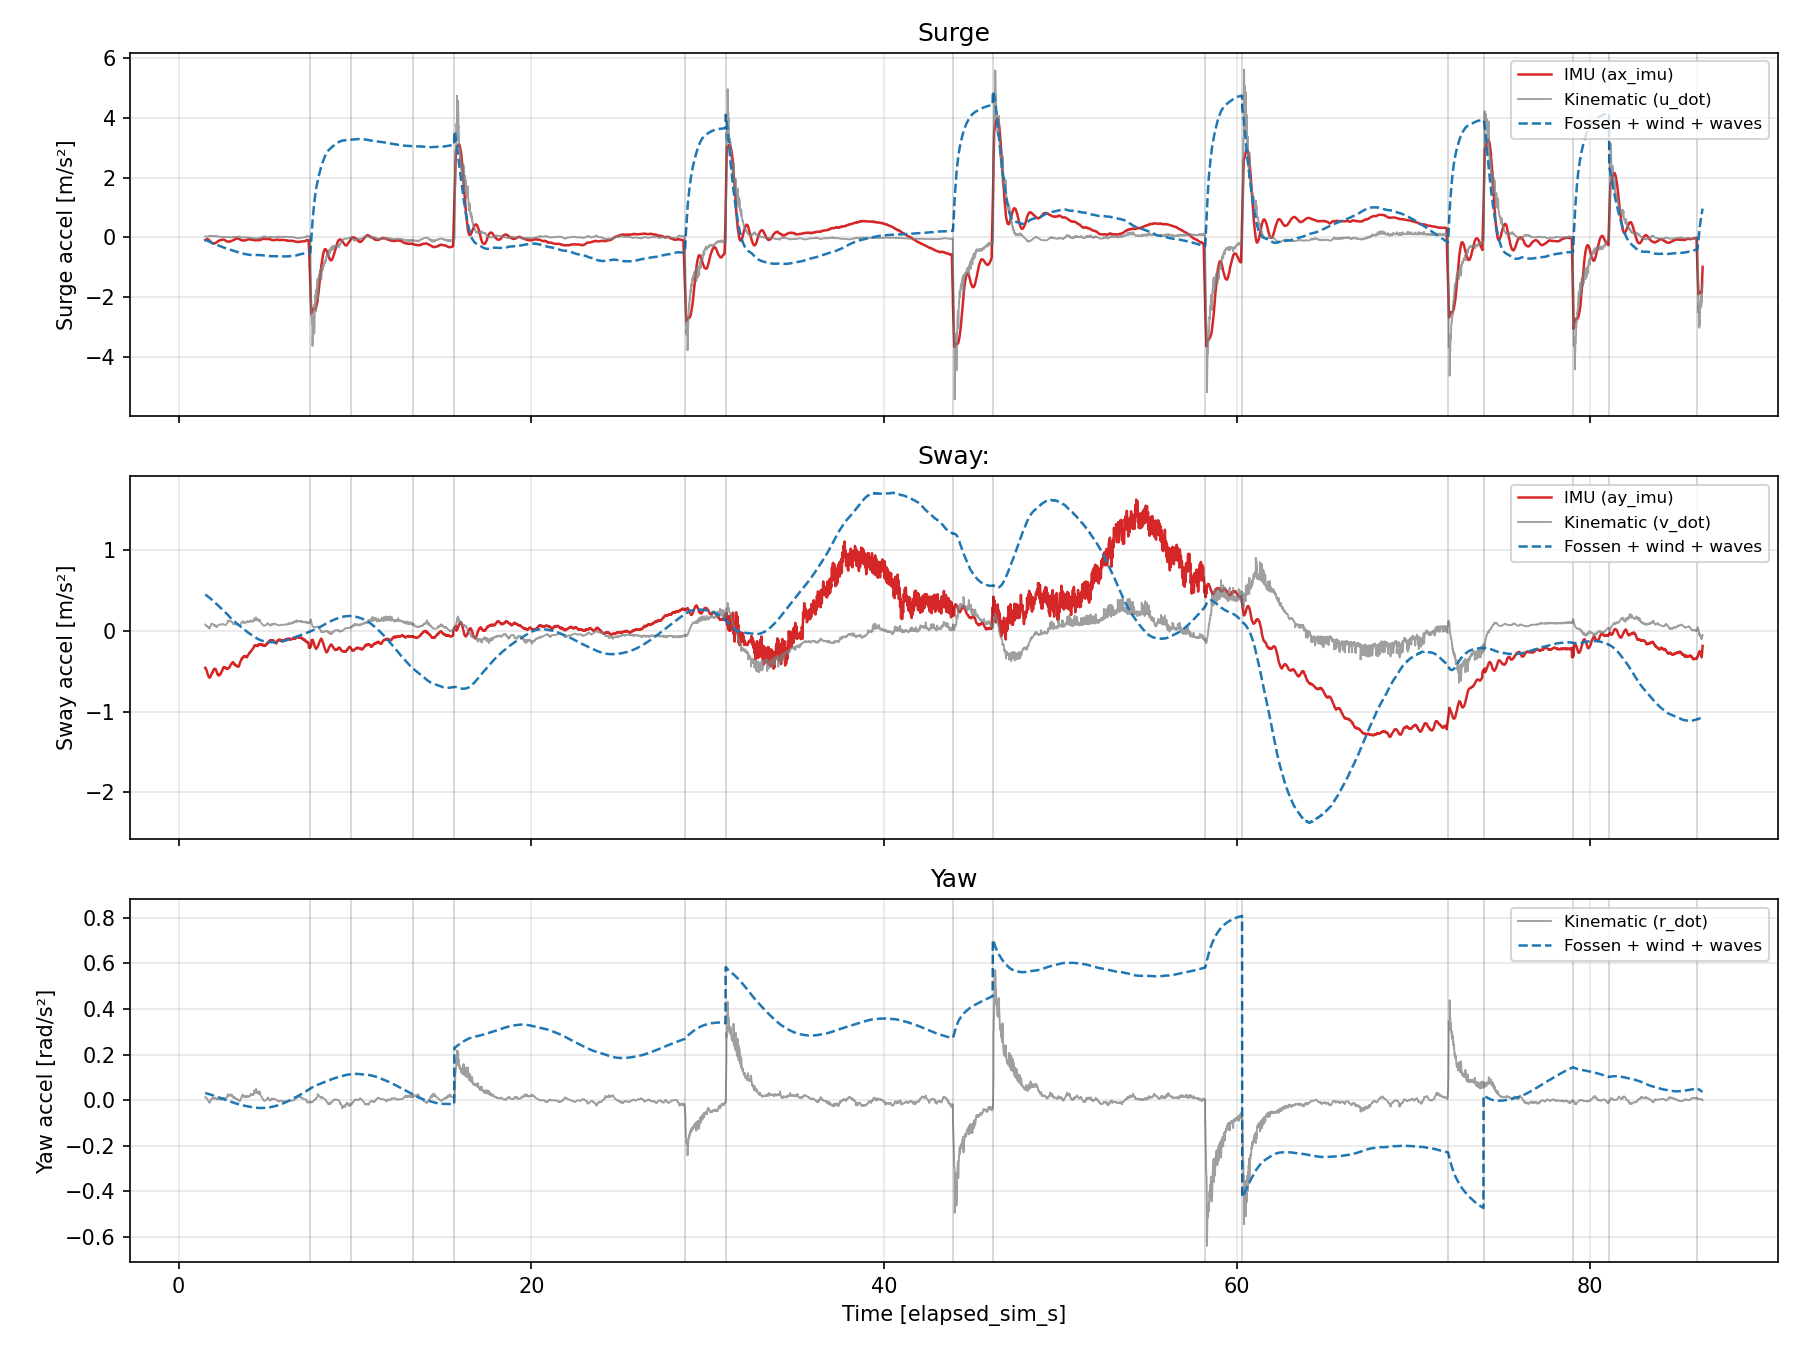
\includegraphics[width=0.8\textwidth]{comparison_essai1.png}
		\caption{Expérience 2 -- accélérations mesurées (IMU, cinématique) et prédites par le modèle}
		\label{fig:exp_1}
	\end{figure}
	
	\paragraph{Indicateurs globaux.}
	Le tableau~\ref{tab:stats_exp_1} résume les statistiques de l'erreur de prédiction
	
	\begin{table}[H]
		\centering
		\caption{Epérience n°2}
		\label{tab:stats_exp_1}
		\begin{tabular}{lcccccc}
			\toprule
			\textbf{Comparaison} & \textbf{Biais} & \textbf{Écart-type} & \textbf{RMSE}
			& \textbf{MAE}\\
			\midrule
			
			$\dot r$ : Fossen $-$ cinématique
			& $+0,184$ & $0,280$ & $0,335$ & $0,265$ \\
			
			$a_x$ : Fossen $-$ IMU
			& $+0,775$ & $1,826$ & $1,984$ & $1,228$\\
			
			$a_y$ : Fossen $-$ IMU
			& $+0,004$ & $0,602$ & $0,602$ & $0,490$\\
			
			\bottomrule
		\end{tabular}
	\end{table}
	
	L’analyse des résultats montre que le comportement du VRX valide globalement la structure du modèle de Fossen en 3~DOF, notamment les vitesses d’équilibre en surge, les couplages de Coriolis et la directionnalité des rotations. Les principales divergences concernent la dynamique transitoire : en surge, le retard de $1$ à $2$~s observé lors des échelons de poussée explique une partie de l’erreur (RMSE $=1{,}984$~m/s²), tandis qu’en sway, la surestimation des accélérations lors des virages (RMSE $=0{,}602$~m/s²) s’explique notamment par la réduction du modèle 6~DOF vers 3~DOF. En yaw, malgré une polarité correctement reproduite, le modèle surestime la réactivité en rotation (RMSE $=0{,}335$~rad/s²), indiquant que l’amortissement hydrodynamique ($N_r,N_{rr}$) est sous-évalué. Ainsi, les écarts observés ne remettent pas en cause la formulation théorique du modèle, mais montrent ses limites quantitatives face aux simplifications du modèle 3~DOF et aux effets dynamiques et stochastiques présents dans l’environnement VRX/Gazebo.
	
	
	
	
	
	\subsection{Validation n°3}
	\label{sec:exp_3}
	
	\paragraph{Paramètres de l'Expérience.}
	% TODO : compléter avec le params.json de cet essai
	Cet expérience reprend les leçons des expériences précédents et les applique à une campagne de
	$N = 14\,986$ échantillons.
	
	\begin{table}[H]
		\centering
		\caption{Expérience 3 -- jeu de paramètres initial}
		\label{tab:params_exp_3}
		\begin{tabular}{ll}
			\toprule
			\textbf{Groupe} & \textbf{Valeurs} \\
			\midrule
			Inertie & $m = 250$~kg, $I_z = 380$~kg·m², $x_g = 0$ \\
			Masse ajoutée & $X_{\dot u} = -100$, $Y_{\dot v} = -80$, $N_{\dot r} = -60$ \\
			Amortissement & $X_u = -50$, $X_{uu} = -180$, $Y_v = -80$, $Y_{vv} = -200$,
			$N_r = -100$, $N_{rr} = -300$ \\
			Propulsion & $k = 1,03$ ; $\ell = 1,0$~m \\
			Vent & $V_w = 15$~m/s, direction $240^\circ$, $(c_x, c_y, c_n) = (0,5;\,0,5;\,0,33)$ \\
			Houle & $T_p = 2$~s, dérive $X = 20$~N, amplitudes $300/300/100$, phases $0$\footnotemark \\
			\bottomrule
		\end{tabular}
	\end{table}
	
	\paragraph{Indicateurs globaux.}
		Rappel méthodologique : le modèle est évalué instantanément à partir des états mesurés
	$(u, v, r)$, sans intégration temporelle ; les courbes du modèle sont donc des restitutions
	instantanées des accélérations, comparées aux mesures IMU et cinématiques (tableau~\ref{tab:stats_exp_3}, figure~\ref{fig:exp_3}).
	
	\begin{table}[H]
		\centering
		\caption{Expérience 3 -- statistiques de l'écart modèle/mesures}
		\label{tab:stats_exp_3}
		\begin{tabular}{lcccccc}
			\toprule
			\textbf{Comparaison} & \textbf{Biais} & \textbf{Écart-type} & \textbf{RMSE}
			& \textbf{MAE} & \textbf{MaxAbsError} \\
			
			\midrule
			
			$\dot r$ : Fossen $-$ cinématique
			& $0,109$ & $0,245$ & $0,268$ & $0,182$
			& $1,094$ \\
			
			$a_x$ : Fossen $-$ IMU
			& $1,427$ & $1,741$ & $2,251$ & $1,586$
			& $6,115$  \\
			
			$a_y$ : Fossen $-$ IMU
			& $0,123$ & $0,354$ & $0,375$ & $0,310$
			& $1,079$  \\
			
			\bottomrule
		\end{tabular}
	\end{table}
	
	\begin{figure}[H]
		\centering
		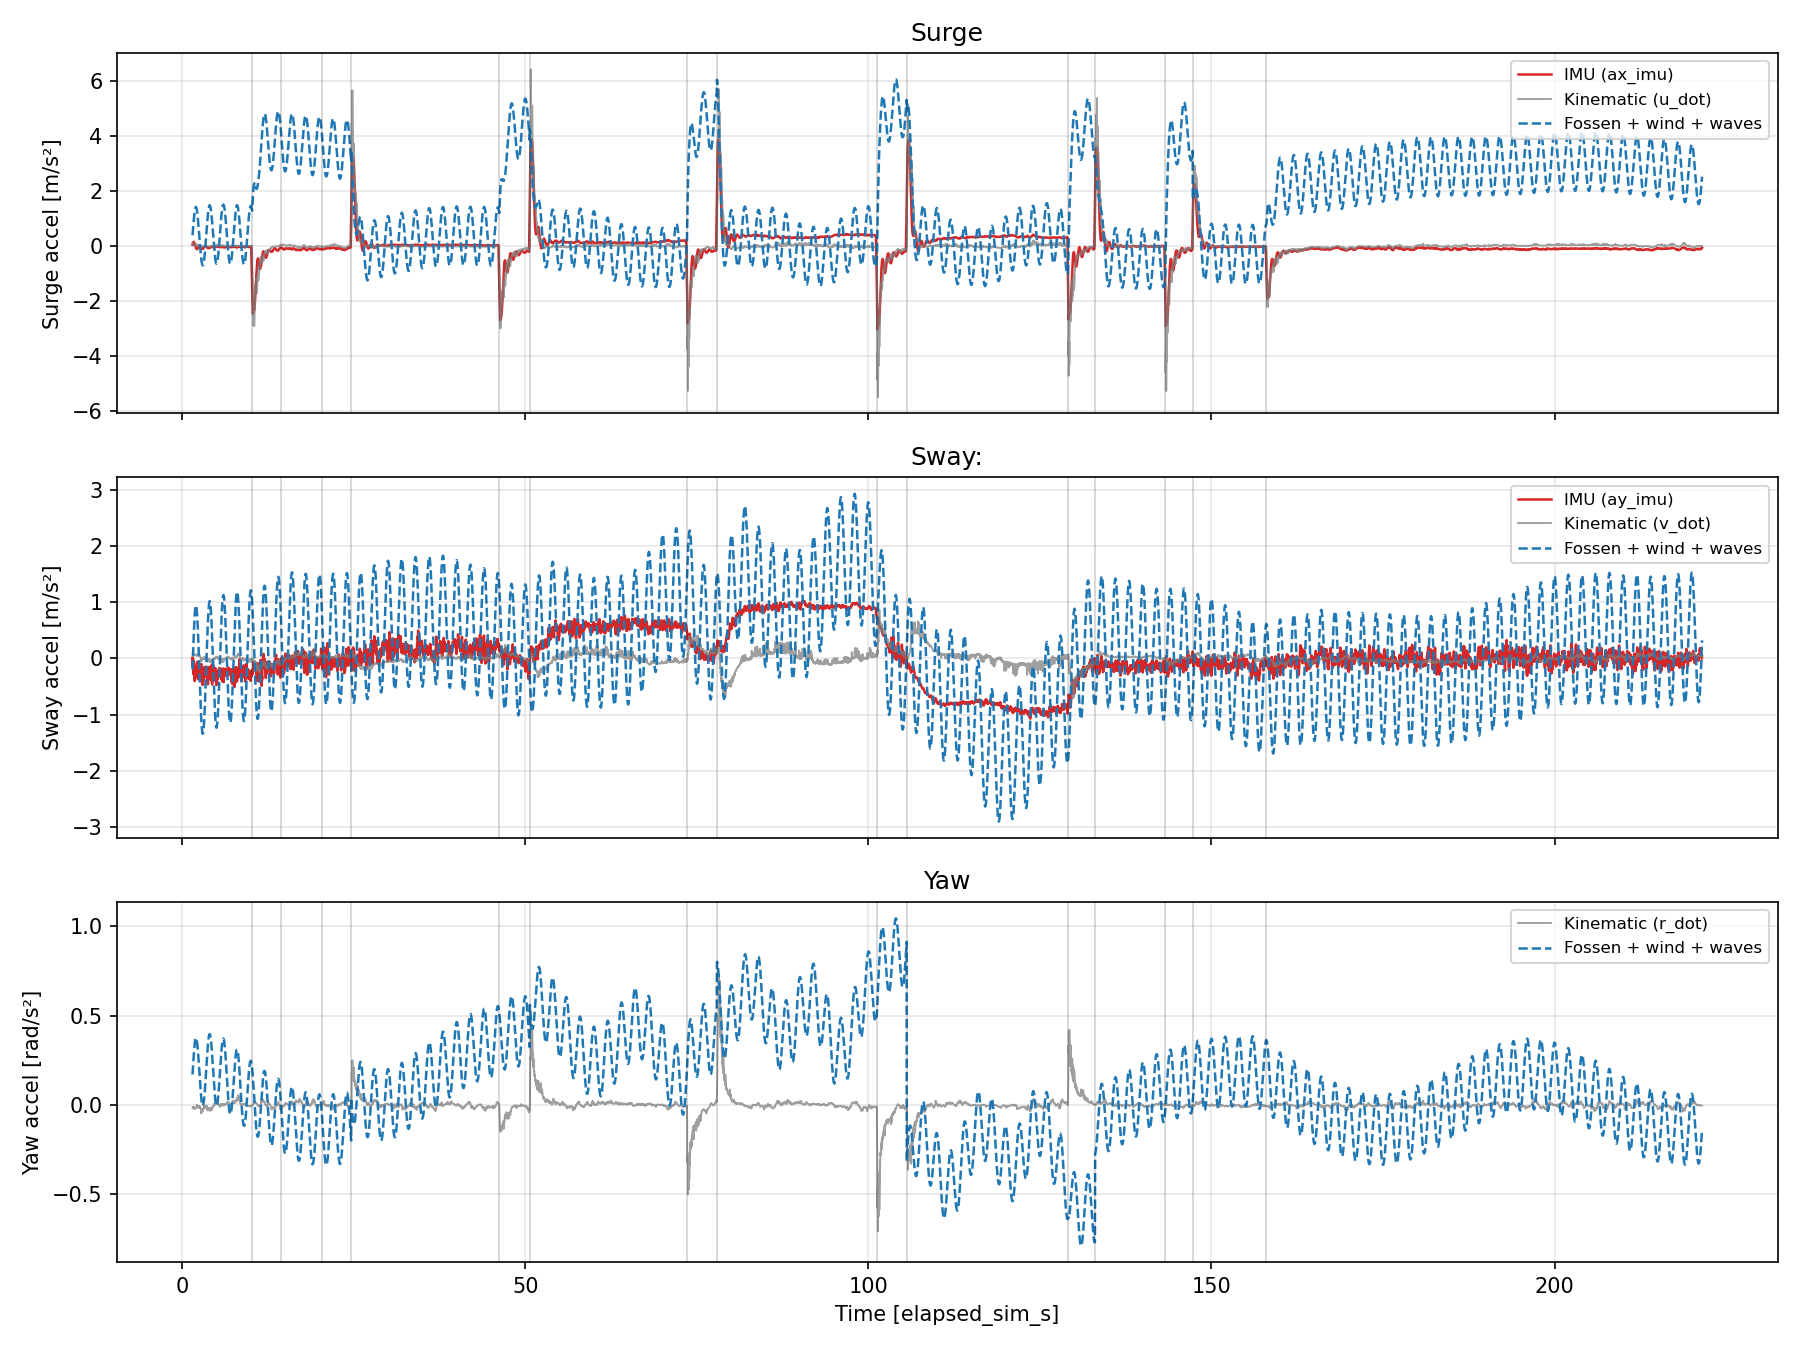
\includegraphics[width=\textwidth]{comparison_essai3.png} % TODO
		\caption{Expérience 4 -- accélérations mesurées (IMU, cinématique) et sorties du modèle de Fossen.}
		\label{fig:exp_3}
	\end{figure}
	
	L’expérience n°3, menée sous des conditions environnementales sévères ($V_w=15$~m/s, $T_p=2$~s), confirme la capacité du modèle de Fossen en 3~DOF à reproduire globalement les dynamiques transversale et rotative du VRX, malgré les perturbations importantes introduites par la houle. L’accord reste satisfaisant en sway (RMSE $=0{,}375$~m/s²) et en yaw (RMSE $=0{,}268$~rad/s²), tandis que l’erreur augmente en surge (RMSE $=2{,}251$~m/s²), où le modèle surestime l’accélération longitudinale lors des régimes permanents et des transitoires. Ces écarts montrent que, malgré une bonne cohérence avec la dynamique globale du VRX, la précision quantitative du modèle reste limitée par les simplifications de la représentation 3~DOF et par les perturbations stochastiques de l’environnement simulé, notamment la houle et les bruits de mesure.
	
	
	% =====================================================
	% TROISIÈME PARTIE : CONCLUSION
	% =====================================================
	\paragraph{Conclusion sur la comparaison des 3 expériences et la validation du modèle.}
	La comparaison synthétique des trois expériences indépendantes permet de porter un jugement clair sur la capacité du modèle de Fossen en 3~DOF à décrire la dynamique du VRX :
	\begin{itemize}[label=--]
		\item \textbf{L'expérience~2}, menée en environnement totalement isolé (vent et houle désactivés), a apporté la preuve décisive de la validité du terme de Coriolis $(m-X_{\dot u})\,u\,r$ en sway, la sortie du modèle épousant parfaitement l'accélération mesurée par l'IMU ($\text{RMSE} = 0{,}253$~m/s²).
		
		\item \textbf{L'expérience~1} a servi de point de référence nominal, confirmant la pertinence de la structure globale du modèle en régime permanent (surge) et en polarité (yaw), tout en isolant des biais spectraux et transitoires.
		
		\item \textbf{L'expérience~3} montre toutefois que, sous des perturbations sévères, les hypothèses du passage du modèle 6~DOF au modèle 3~DOF sont dépassées, limitant ainsi la précision du modèle réduit.
		
	\end{itemize}
	
	En synthèse, ces travaux valident la structure algébrique et théorique du modèle de Fossen en 3~DOF pour représenter le comportement plan du VRX. Néanmoins, sa validité quantitative globale reste partielle sous sa formulation idéale actuelle. Les divergences observées ne remettent pas en cause la formulation mathématique elle-même, mais définissent ses limites d'application face à deux facteurs critiques principaux: (i)~les simplifications inhérentes à la réduction 3~DOF et les simplifications du modèle où il suit juste le mouvement selon surge, sway et yaw et (ii)~le caractère stochastique de l'environnement sous Gazebo (bruits capteurs, variations aléatoires de la houle et du vent).
	
	\newpage
	
	% =====================================================
	% TROISIÈME PARTIE : GUIDAGE ET CONTRÔLE DU CATAMARAN
	% =====================================================
	\section{Guidage du catamaran}
	\label{sec:guidage}
	
	La validation du modèle dynamique (Partie~2) constitue le prérequis indispensable au développement des lois de commande. L'objectif final du projet est la navigation vers les déchets, le catamaran doit être capable de naviguer de manière autonome entre des points d'intérêt définis, en compensant les perturbations environnementales. Cette partie détaille l'architecture logicielle, la loi de guidage proportionnelle mise en œuvre et les résultats obtenus en simulation.
	
	\begin{figure}[H]
		\centering

		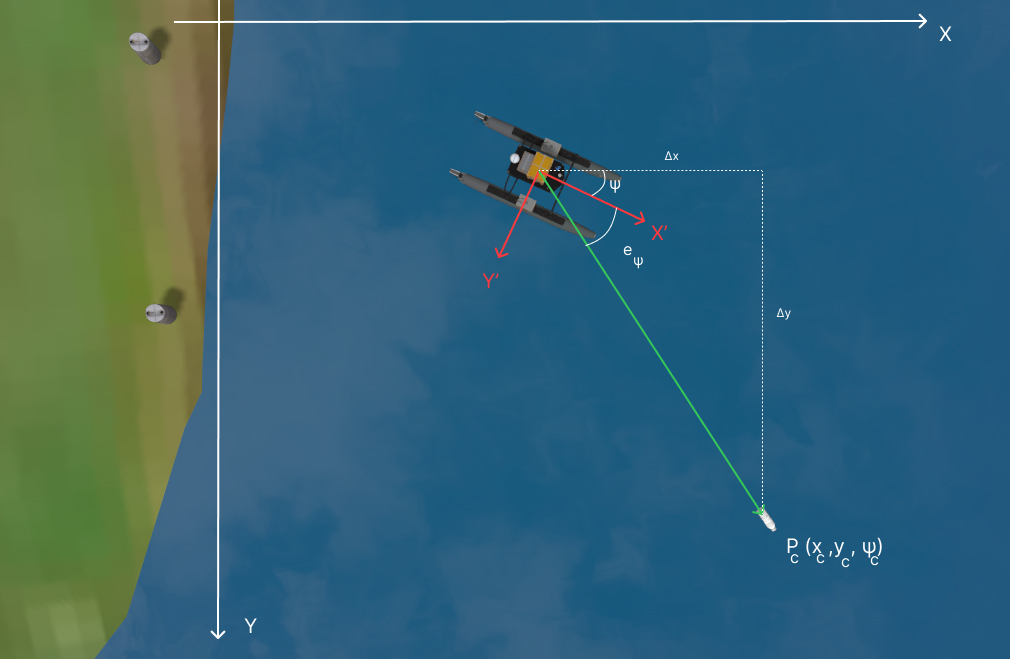
\includegraphics[width=0.8\textwidth]{guide.jpg} 
		\caption{Le but est d'arriver au point cible (déchet).}
		\label{fig:dechet}
	\end{figure}
	
	\subsection{Stratégie de guidage: Commande proportionnelle}
	Pour assurer la navigation point à point, nous avons implémenté une loi de guidage proportionnelle, couplée à un contrôleur proportionnel en cap. Le principe est de calculer en temps réel le cap désiré $\psi_c$ pointant vers la cible actuelle $P_c(x_c, y_c, \psi_c)$, puis de générer des commandes de propulsion pour annuler l'erreur de cap $e_\psi$.
	
	Soit $(x, y)$ la position actuelle du catamaran dans le repère local. Le vecteur d'erreur de position s'écrit :
	\begin{equation}
		\Delta x = x_c - x, \quad \Delta y = y_c - y
	\end{equation}
	La distance euclidienne au waypoint est donnée par $d = \sqrt{\Delta x^2 + \Delta y^2}$. Le cap désiré est ensuite calculé via la fonction à quatre quadrants :
	\begin{equation}
		\psi_c = \mathrm{atan2}(\Delta y, \Delta x)
	\end{equation}
	Afin d'éviter les discontinuités lors du passage de $+\pi$ à $-\pi$, l'erreur de cap $e_\psi$ est normalisée dans l'intervalle $[-\pi, \pi]$ à l'aide d'une fonction de wrapping :
	\begin{equation}
		e_\psi = \psi_c - \psi
	\end{equation}
	
	\subsection{Architecture logicielle du flux de guidage}
	L'implémentation repose sur un nœud ROS~2 dédié, qui s'exécute à une fréquence de 20~Hz. Ce nœud souscrit aux topics de localisation et publie les consignes de poussée vers les propulseurs. Le diagramme de la figure~\ref{fig:flux_guidage} synthétise le flux de données et les décisions logiques.
	
	
	% --- DÉBUT DU DIAGRAMME TIKZ ADAPTÉ ---
	\begin{figure}[H]
		\centering
		\resizebox{\textwidth}{!}{%
			\begin{tikzpicture}[
				node distance=0.7cm and 1.0cm,
				font=\small\sffamily,
				block/.style={draw, rectangle, rounded corners=3pt, align=center, inner sep=5pt, fill=white, text width=5.0cm},
				blueblock/.style={block, draw=blueframe, fill=white},
				orangeblock/.style={block, draw=orangeframe, fill=white},
				pinkblock/.style={block, draw=pinkframe, fill=white},
				purpleblock/.style={block, draw=purpleframe, fill=white},
				decision/.style={draw=blueframe, diamond, aspect=2.2, align=center, fill=white, inner sep=3pt, font=\small, text width=2.6cm},
				line/.style={draw, -{Stealth[length=2.5mm]}, thick, gray!80!black},
				infobox/.style={draw=blueframe, dashed, rounded corners=5pt, fill=bluebg!30, inner sep=6pt, text width=5.6cm, font=\footnotesize, align=left}
				]
				
				% ==========================================
				% COLONNE 1
				% ==========================================
				\node[blueblock] (gps) {
					\textbf{GPS}\\[2pt]
					\scriptsize(Latitude, Longitude)\\
					\textbf{IMU}\\[2pt]
					\scriptsize (Accélérations, Vitesses angulaires)
					
				};
				
				
				
				\node[blueblock, fill=bluebg!50, below=1.6cm of gps] (sorties) {
					\textbf{Sorties}\\[3pt]
					\scriptsize $\bullet$ Position $(x, y)$\\[2pt]
					\scriptsize $\bullet$ Cap ($\psi$)
				};
				
				% ==========================================
				% COLONNE 2
				% ==========================================
				\node[orangeblock, right=1.0cm of gps] (w_actif) {
					\textbf{Cible $P_c(x_c, y_c)$}\\[2pt]
				};
				
				\node[orangeblock, below=0.9cm of w_actif] (v_erreur) {
					\textbf{Vecteur d'erreur}\\[2pt]
					$\Delta x = x_c - x$\\[2pt]
					$\Delta y = y_c - y$
				};
				
				\node[orangeblock, below=0.9cm of v_erreur] (dist) {
					\textbf{Distance au waypoint}\\[2pt]
					$d = \sqrt{\Delta x^2 + \Delta y^2}$
				};
				
				\node[orangeblock, below=0.9cm of dist] (cap_des) {
					\textbf{Cap désiré (ligne de visée)}\\[2pt]
					$\psi_c = \mathrm{atan2}(\Delta y, \Delta x)$
				};
				
				\node[orangeblock, below=0.9cm of cap_des] (err_cap) {
					\textbf{Erreur de cap}\\[2pt]
					$e_\psi = \psi_c - \psi$\\[2pt]
					\tiny ($-\pi \le e_\psi \le \pi$)
				};
				
				\node[decision, below=0.7cm of err_cap] (dec_dist) {
					$d \le 1\text{ m ?}$\\[2pt]
				};
				
				\node[block, draw=greenframe, fill=greenbg, below=0.7cm of dec_dist] (w_atteint) {
					\textbf{Cible atteinte}\\[2pt]
					\scriptsize Passage automatique au\\ waypoint suivant
				};
				
				% ==========================================
				% COLONNE 3
				% ==========================================
				\node[pinkblock, right=1.0cm of w_actif] (cmd_prop) {
					\scriptsize Commande proportionnelle\\[2pt]
					$T_\Delta = K_p \cdot e_\psi$\\[2pt]
					\tiny ($K_p = 300$)
				};
				
				\node[pinkblock, below=0.9cm of cmd_prop] (repartition) {
					\textbf{\scriptsize Répartition des poussées}\\[2pt]
					$T_L = T_{\text{base}} - T_\Delta$\\[2pt]
					$T_R = T_{\text{base}} + T_\Delta$
				};
				
				
				\node[purpleblock, dashed, fill=purplebg!40, below=0.9cm of repartition] (pub) {
					\textbf{\scriptsize Publication des commandes}\\[2pt]
					\scriptsize $T_L \rightarrow \texttt{/left\_thruster\_cmd}$\\[2pt]
					\scriptsize $T_R \rightarrow \texttt{/right\_thruster\_cmd}$
				};
				
				% ==========================================
				% ACTIONNEUR
				% ==========================================
				\node[purpleblock, fill=purplebg!60, below=0.8cm of pub, text width=6cm] (usv_action) {
					\textbf{4. ACTION SUR LE DRONE}\\[2pt]
					\scriptsize \textbf{Propulseurs}\\[2pt]
					\scriptsize Application de $T_L$ et $T_R \rightarrow$ Mouvement
				};
				
				% ==========================================
				% ENCARTS DROITE
				% ==========================================
				\node[infobox, right=1.0cm of cmd_prop, anchor=north west] (eq_cles) {
					\centering \textbf{\textcolor{blue!60!black}{ÉQUATIONS CLÉS}}\\[4pt]
					$\bullet$ \textbf{Vecteur d'erreur :} $\Delta x = x_d - x$, $\Delta y = y_d - y$\\[3pt]
					$\bullet$ \textbf{Distance :} $d = \sqrt{\Delta x^2 + \Delta y^2}$\\[3pt]
					$\bullet$ \textbf{Cap désiré :} $\psi_d = \mathrm{atan2}(\Delta y, \Delta x)$\\[3pt]
					$\bullet$ \textbf{Erreur de cap :} $e_\psi = \mathrm{wrapToPi}(\psi_d - \psi)$\\[3pt]
					$\bullet$ \textbf{Commande prop. :} $T_\Delta = K_p \cdot e_\psi$\\[3pt]
					$\bullet$ \textbf{Commandes moteurs :}\\[1pt]
					\quad $T_L = T_{\text{base}} - T_\Delta$, \; $T_R = T_{\text{base}} + T_\Delta$
				};
				
				\node[infobox, below=0.6cm of eq_cles.south west, anchor=north west] (interp) {
					\centering \textbf{\textcolor{blue!60!black}{INTERPRÉTATION}}\\[4pt]
					$\bullet$ $T_{\text{base}}$ contrôle l'avance (vitesse)\\[3pt]
					$\bullet$ $T_\Delta$ crée la différence de poussée pour tourner\\[3pt]
					$\bullet$ $K_p$ règle la réactivité du cap\\[3pt]
					$\bullet$ Plus $|e_\psi|$ est grand, plus la diff. de poussée est grande\\[3pt]
				};
				
				% ==========================================
				% BACKGROUND GROUPS
				% ==========================================
				\begin{scope}[on background layer]
					\node[fit=(gps)(sorties), draw=blueframe, fill=bluebg!30, rounded corners=5pt, inner sep=8pt] (box1) {};
					\node[anchor=south, font=\bfseries\color{blue!50!black}\footnotesize] at (box1.north) {1. ACQUISITION DES DONNÉES};
					
					\node[fit=(w_actif)(w_atteint), draw=orangeframe, fill=orangebg!30, rounded corners=5pt, inner sep=8pt] (box2) {};
					\node[anchor=south, font=\bfseries\color{orange!80!black}\footnotesize] at (box2.north) {2. GUIDAGE};
					
					\node[fit=(cmd_prop)(pub), draw=pinkframe, fill=pinkbg!30, rounded corners=5pt, inner sep=8pt] (box3) {};
					\node[anchor=south, font=\bfseries\color{pink!50!black}\footnotesize, align=center] at (box3.north) {3. CONTRÔLE PROPORTIONNELLE};
				\end{scope}
				
				% ==========================================
				% FLÈCHES
				% ==========================================
				\draw[line] (gps) -- (sorties);
				\draw[line] (sorties.east) -- ++(0.5,0) |- (v_erreur.west);
				\draw[line] (w_actif) -- (v_erreur);
				\draw[line] (v_erreur) -- (dist);
				\draw[line] (dist) -- (cap_des);
				\draw[line] (cap_des) -- (err_cap);
				\draw[line] (err_cap) -- (dec_dist);
				\draw[line] (dec_dist) -- node[right, font=\bfseries\tiny, color=green!50!black]{OUI} (w_atteint);
				
				% Flèche NON : contourne par la gauche sans traverser les blocs
				\draw[line] (dec_dist.west) -- node[above, font=\bfseries\tiny, color=red]{NON} ++(-3.5,0) 
				-| (sorties.south);
				
				\draw[line] (box2.east |- cmd_prop.west) -- (cmd_prop.west);
				\draw[line] (cmd_prop) -- (repartition);
				\draw[line] (repartition) -- (pub);
				\draw[line] (pub) -- (pub |- usv_action.north);
				
			\end{tikzpicture}
		}
		\caption{Flux de données et logique de décision du nœud de guidage proportionnel.}
		\label{fig:flux_guidage}
	\end{figure}
	% --- FIN DU DIAGRAMME TIKZ ---
	
	\subsection{Loi de commande et répartition des poussées}
	Le cœur du contrôleur réside dans la transformation de l'erreur de cap $e_\psi$ en une différence de poussée $T_\Delta$ entre les propulseurs bâbord ($T_L$) et tribord ($T_R$). La loi de commande proportionnelle s'écrit :
	\begin{equation}
		T_\Delta = K_p \cdot e_\psi
	\end{equation}
	où $K_p$ est le gain proportionnel (réglé empiriquement à $K_p = 300$ lors de nos tests pour offrir un compromis entre réactivité et stabilité). 
	
	La consigne finale pour chaque propulseur est calculée en superposant une poussée de base $T_{\text{base}}$ (assurant l'avancement) et la correction directionnelle $T_\Delta$ :
	\begin{equation}
		T_L = \mathrm{sat}(T_{\text{base}} - T_\Delta, 0, T_{\max}), \quad
		T_R = \mathrm{sat}(T_{\text{base}} + T_\Delta, 0, T_{\max})
	\end{equation}
	

	\subsection{Résultats de simulation et analyse}
	Pour évaluer les performances du guidage, un scénario de navigation passant par quatre waypoints formant un rectangle a été exécuté dans le monde \texttt{sydney\_regatta}, avec des conditions de vent modérées ($V_w = 5$~m/s) et les vagues sont désactivées.
	
	\begin{figure}[H]
		\centering
		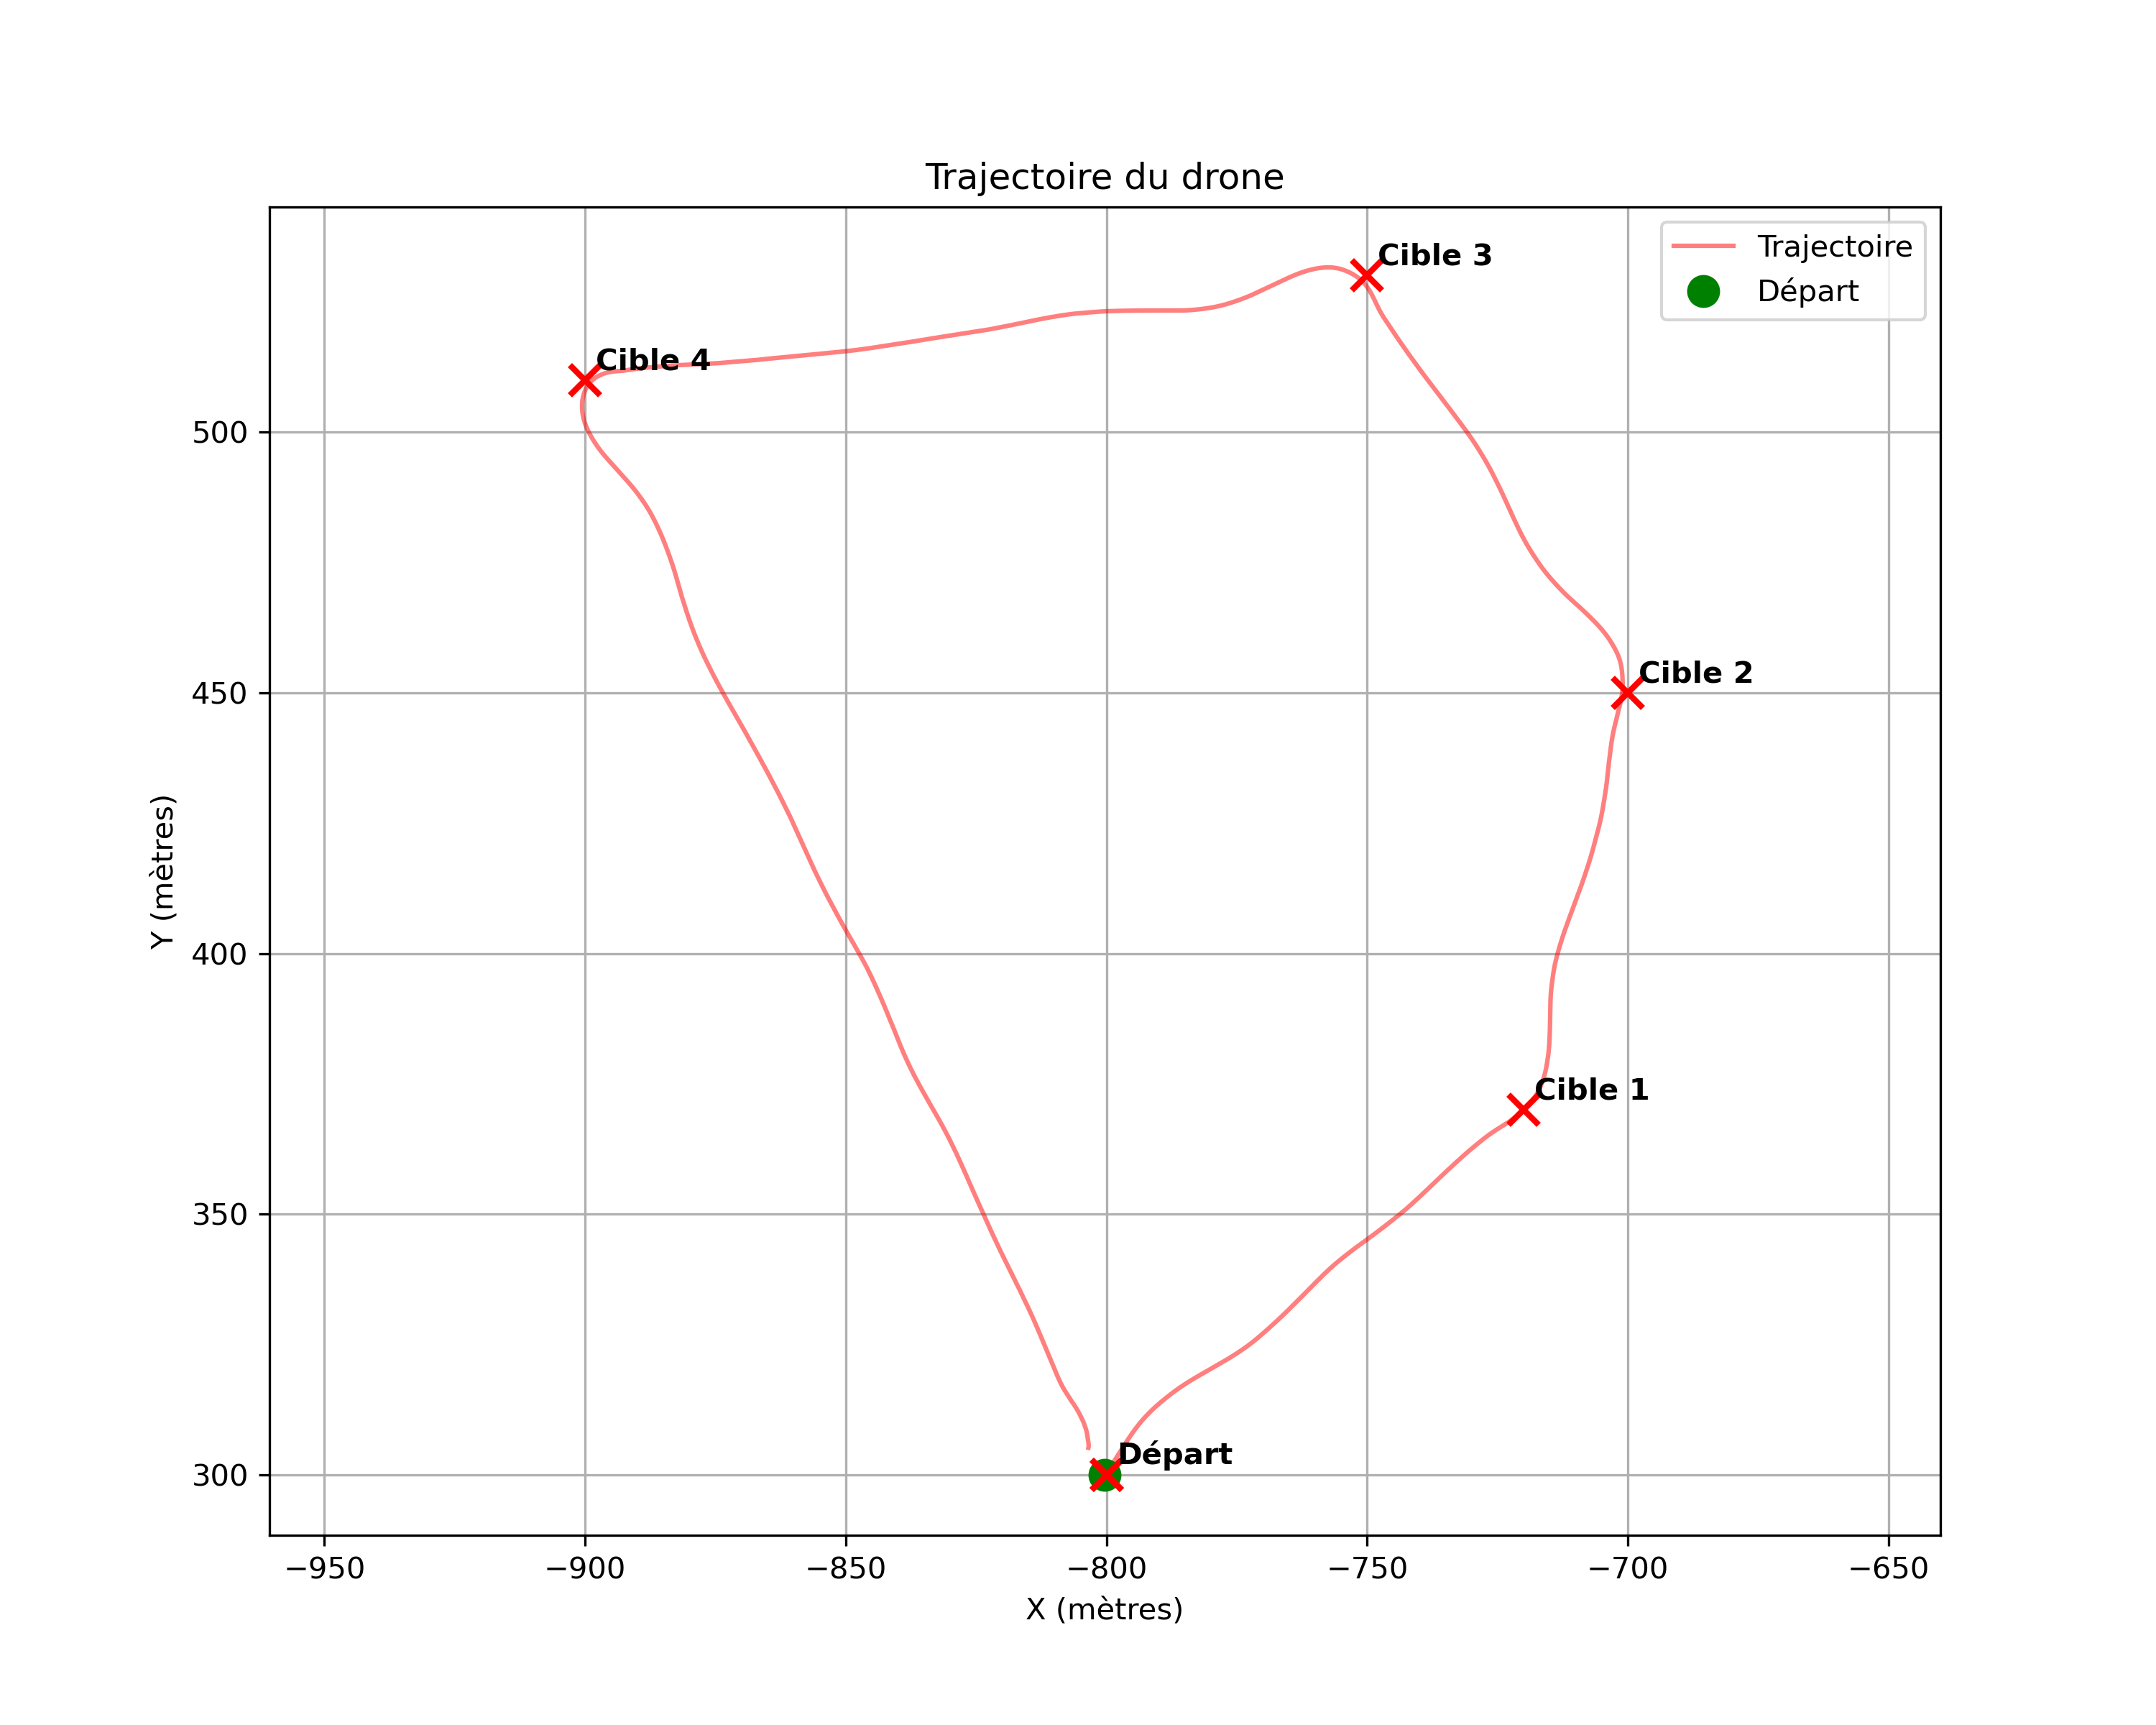
\includegraphics[width=0.8\textwidth]{trajectoire_multipoint.png} 
		\caption{Trajectoire suivie par le catamaran lors de la navigation multi-waypoints }
		\label{fig:traj_guidage}
	\end{figure}
	
	L'analyse de la figure~\ref{fig:traj_guidage} et des journaux d'exécution révèle plusieurs points clés :
	\begin{itemize}[label=--]
		\item \textbf{Convergence vers la ligne de visée :} Après chaque changement de waypoint, le catamaran effectue un virage coordonné pour aligner son cap $\psi$ sur $\psi_c$. La poussée différentielle permet une rotation sur place efficace, validant le couplage lacet-propulsion du modèle.
		\item \textbf{Erreur de cap en régime permanent :} En ligne droite, l'erreur $e_\psi$ oscille autour de zéro avec une amplitude maximale de $\pm 0{,}15$~rad. Cette légère oscillation est inhérente au contrôleur purement proportionnel face aux perturbations stochastiques de la houle.
		\item \textbf{Validation du seuil de basculement :} Le rayon de $1$~m s'est avéré adapté. Le drone ne présente pas d'oscillations excessives au voisinage des waypoints et enchaîne les segments de manière fluide.
	\end{itemize}
	

	
	
	\section{Conclusion générale}
	\label{sec:conclusion}
	
	Ce stage avait pour objectif de développer et de valider un environnement de simulation pour un drone de surface autonome (USV), destiné à constituer une base pour le développement ultérieur de systèmes de navigation et de collecte autonome de déchets marins. L'environnement mis en place repose sur l'association de ROS~2, Gazebo et du framework VRX, permettant de reproduire un environnement maritime dynamique intégrant notamment les effets du vent et de la houle. Cette plateforme fournit ainsi un cadre expérimental permettant de tester différentes stratégies de guidage et de commande sans avoir recours immédiatement au véhicule réel.
	
	Une première contribution importante du travail réalisé concerne la mise en œuvre d'une chaîne complète d'acquisition et de traitement des données issues de la simulation. Les informations provenant de la pose, de l'IMU et des propulseurs ont été enregistrées et exploitées afin d'estimer les variables dynamiques du véhicule. La validation du modèle de Fossen à trois degrés de liberté a ensuite permis de vérifier la cohérence entre les accélérations prédites par le modèle et celles obtenues à partir de la simulation. Le protocole expérimental mis en place, reposant sur différentes excitations en translation et en rotation, a permis d'explorer plusieurs régimes de fonctionnement du catamaran et de mettre en évidence les écarts liés notamment aux paramètres hydrodynamiques et à la dynamique des actionneurs.
	
	La seconde contribution concerne le développement d'une première stratégie de guidage point à point. Une loi de guidage proportionnelle associée à une commande différentielle des deux propulseurs a permis au catamaran de rejoindre les différentes cibles dans l'environnement simulé. Cette approche constitue une première étape vers l'autonomie du véhicule. Toutefois, les expérimentations ont également montré les limites d'une commande purement proportionnelle, notamment en présence de perturbations persistantes et lors de variations importantes du comportement dynamique du véhicule. En particulier, le réglage fixe du gain $K_p$ impose un compromis entre rapidité de réaction et stabilité, tandis qu'une perturbation constante peut conduire à une erreur résiduelle. Ces limites motivent naturellement l'évolution vers des stratégies de commande plus robustes.
	
	\section{Perspectives}
	
	Les travaux réalisés constituent ainsi une première brique d'une architecture plus complète de guidage, navigation et contrôle. Plusieurs axes d'amélioration peuvent être envisagés.
	

	Une première évolution consiste à remplacer le contrôleur proportionnel actuel par une commande PID ou, plus généralement, par une loi de commande permettant de mieux compenser les perturbations et les erreurs persistantes. L'ajout d'une action intégrale permettrait notamment de réduire l'erreur statique en présence de perturbations constantes. Une loi de guidage LOS plus avancée, prenant explicitement en compte l'erreur transversale (\emph{cross-track error}), permettrait également d'améliorer le suivi des trajectoires et la précision d'approche des déchets.
	

	À plus long terme, une approche fondée sur la commande prédictive par modèle (MPC) pourrait être étudiée. Contrairement à une commande réactive classique, le MPC exploiterait le modèle dynamique du véhicule afin de prédire son évolution sur un horizon temporel et de déterminer les commandes optimales tout en respectant les contraintes sur les propulseurs, la vitesse et les changements de cap. Cette approche serait particulièrement intéressante dans un environnement maritime soumis simultanément au vent, à la houle et aux courants, où les effets des perturbations doivent être anticipés plutôt que simplement corrigés après leur apparition.
	

	L'amélioration du système de navigation constitue également une perspective importante. Les états du véhicule pourraient être estimés à partir de la fusion des informations provenant du GPS, de l'IMU, du LiDAR et, à terme, de la caméra. Un filtre de Kalman étendu (EKF) ou un filtre de Kalman unscented (UKF) pourrait être intégré afin d'obtenir une estimation plus robuste de la position, de l'orientation, des vitesses et des perturbations subies par le véhicule. Cette estimation permettrait de réduire la dépendance à une mesure unique et fournirait au contrôleur un état plus fiable du système.
	

	Une autre perspective consiste à rendre la commande adaptative grâce à des méthodes d'apprentissage automatique. Les paramètres hydrodynamiques du modèle, tels que les coefficients d'amortissement ou certains termes associés aux perturbations, pourraient être estimés en ligne à partir des données collectées. Le contrôleur pourrait ainsi adapter progressivement son comportement aux variations des conditions de navigation. Cette approche permettrait notamment de prendre en compte les changements de régime liés à la vitesse du véhicule, à la direction du vent ou aux caractéristiques de la houle.
	

	Une évolution plus ambitieuse serait l'intégration de méthodes d'apprentissage par renforcement (RL) pour apprendre directement une politique de commande à partir des interactions avec l'environnement simulé. La plateforme VRX constitue à ce titre un environnement particulièrement intéressant pour entraîner et comparer différentes politiques avant leur éventuel transfert vers un véhicule réel. Des méthodes telles que SAC, TD3 ou PPO pourraient être étudiées pour apprendre des stratégies de commande robustes face aux perturbations et aux différentes configurations de navigation.
	

	Enfin, l'étape ultime du projet consiste à dépasser le simple guidage point à point afin de réaliser une mission complète de collecte autonome. Le système devra alors combiner plusieurs niveaux : perception des déchets par caméra et LiDAR, estimation de leur position, planification de trajectoire, évitement des obstacles, guidage vers la cible et commande robuste du véhicule. La plateforme développée durant ce stage pourra servir de socle pour tester progressivement ces différentes briques et évaluer leur comportement dans des conditions environnementales contrôlées.
	
	Ainsi, le travail réalisé ne constitue pas une solution finale de navigation autonome, mais fournit une base expérimentale et logicielle permettant d'aborder progressivement des stratégies de contrôle plus avancées. L'évolution d'une commande proportionnelle vers une architecture intégrant estimation d'état, adaptation par apprentissage, commande prédictive et, à terme, apprentissage par renforcement représente une perspective naturelle pour rendre le système plus autonome, robuste et capable de fonctionner dans des environnements maritimes fortement perturbés.
	
	
	\newpage
	% ==================== BIBLIOGRAPHIE ====================
	\begin{thebibliography}{9}
		\addcontentsline{toc}{section}{Bibliographie}
		
		\bibitem{atron} J.~Abanes, H.~Jang, B.~Erkinov, J.~Awadalla et A.~Tzes,
		\og ATRON : Autonomous trash retrieval for oceanic neatness\fg,
		\emph{Frontiers in Robotics and AI}, vol.~12, 1718177, 2026.
		DOI : 10.3389/frobt.2025.1718177
		
		\bibitem{vrx} B.~Bingham et al.,
		\og Toward maritime robotic simulation in Gazebo\fg,
		in \emph{Proc. OCEANS 2019 MTS/IEEE SEATTLE}, pp.~1--10, 2019.
		DOI : 10.23919/OCEANS40490.2019.8962724
		
		\bibitem{vrx2} B.~Saldarriaga-Mesa, J.~Montesdeoca, D.~Báez, F.~Roberti et J.~M.~Toibero,
		\og Open-Access Simulation Platform and Motion Control Design for a Surface Robotic Vehicle in the VRX Environment\fg,
		\emph{Robotics}, vol.~14, no.~10, p.~147, 2025.
		DOI : 10.3390/robotics14100147
		
		\bibitem{rantala} A.~Rantala,
		\emph{Design Principles of ROS~2 Based Autonomous Shipping Systems},
		thèse de doctorat, Université de Jyväskylä, 2025.
		
		\bibitem{lebars}
		F.~Le Bars et L.~Jaulin,
		\emph{Robotic Sailing 2013},
		Springer, 2013.
		
		\bibitem{jaulin_etat}
		L.~Jaulin,
		\emph{Représentation d'état pour la modélisation et la commande des systèmes},
		2013.
		
		\bibitem{saoud}
		H.~Saoud,
		\emph{Modélisation et commande de voiliers autonomes},
		Thèse de doctorat, Université de Bretagne Occidentale, 2013.
		
		\bibitem{fossen}
		T.~I.~Fossen,
		\emph{Handbook of Marine Craft Hydrodynamics and Motion Control},
		Wiley, Chichester, 2011.
		
		\bibitem{sname}
		E.~V.~Lewis (ed.),
		\emph{Principles of Naval Architecture, Volume III:
			Motions in Waves and Controllability},
		Society of Naval Architects and Marine Engineers (SNAME),
		1989.
		
		\bibitem{bingham19toward}
		B.~Bingham, C.~Aguero, M.~McCarrin, J.~Klamo, J.~Malia,
		K.~Allen, T.~Lum, M.~Rawson et R.~Waqar,
		``Toward Maritime Robotic Simulation in Gazebo,''
		\emph{Proceedings of the MTS/IEEE OCEANS Conference},
		Seattle, WA, USA, 2019.
		
		\bibitem{github} GitHub: \href{https://github.com/oussamaissm/Development-of-a-Simulation-Environment-for-an-Unmanned-Surface-Vehicle-USV-}{\emph{Development of a Simulation Environment for an Unmanned Surface Vehicle (USV)}}, 2026.
		
	\end{thebibliography}
	
	% =====================================================
	% QUATRIÈME PARTIE : ANNEXES
	% =====================================================
	\begin{appendix}
		
		
		
		
		
		\section{Glossaire des variables du modèle de Fossen 3-DOF}
		\label{ann:glossaire}
		Le tableau~\ref{tab:glossaire} rassemble, pour référence rapide, l'ensemble des symboles utilisés dans
		la section~\ref{sec:fossen}.
		
		\begin{table}[H]
			\centering
			\caption{Glossaire des principales variables du modèle 3-DOF}
			\label{tab:glossaire}
			\begin{tabular}{ll}
				\toprule
				\textbf{Symbole} & \textbf{Signification} \\
				\midrule
				$u, v, r$ & vitesses de surge, sway et lacet (repère corps) \\
				$\dot u, \dot v, \dot r$ & accélérations correspondantes \\
				$\psi$ & cap du véhicule \\
				$T_L, T_R$ & consignes de poussée gauche et droite \\
				$\tau = [X, Y, N]^\top$ & torseur des forces généralisées (surge, sway, lacet) \\
				$m$, $x_g$, $I_z$ & masse, abscisse du centre de gravité, inertie en lacet \\
				$X_{\dot u}, Y_{\dot v}, Y_{\dot r}, N_{\dot v}, N_{\dot r}$ & masses ajoutées \\
				$X_u, X_{uu}, Y_v, Y_{vv}, N_r, N_{rr}$ & coefficients d'amortissement linéaire/quadratique \\
				$V_w, \beta$ & vitesse et direction du vent \\
				$c_x, c_y, c_n$ & coefficients aérodynamiques ducatamaran \\
				$T_p, \omega_p$ & période pic et pulsation associée du vent \\
				\bottomrule
			\end{tabular}
		\end{table}
		

		\section{Relations mathématiques implantées dans les codes}
		\label{app:formulaires}
		
		\subsection{Mesures et prétraitements}
		\label{app:mesures}
		
		
		Attitude extraite d'un quaternion normalisé $q=(x,y,z,w)$ :
		\begin{align}
			\psi    &= \mathrm{atan2}\big(2(wz+xy),\ 1-2(y^{2}+z^{2})\big) \label{eq:yaw}\\
			\phi    &= \mathrm{atan2}\big(2(wx+yz),\ 1-2(x^{2}+y^{2})\big) \label{eq:roll}\\
			\theta  &= \mathrm{asin}\big(2(wy-zx)\big)                    \label{eq:pitch}
		\end{align}
		
		Recentrage sur la première pose $(x_{0},y_{0},\psi_{0})$ :
		\begin{equation}
			\begin{aligned}
				x_{\mathrm{loc}} &= \phantom{-}(x-x_{0})\cos\psi_{0} + (y-y_{0})\sin\psi_{0}\\
				y_{\mathrm{loc}} &= -(x-x_{0})\sin\psi_{0} + (y-y_{0})\cos\psi_{0}\\
				\psi_{\mathrm{loc}} &= \mathrm{wrap}(\psi-\psi_{0})
			\end{aligned}
			\label{eq:local}
		\end{equation}
		
		Vitesses monde par différences finies :
		\begin{equation}
			\dot{x} = \frac{x_{k}-x_{k-1}}{\Delta t},\quad
			\dot{y} = \frac{y_{k}-y_{k-1}}{\Delta t},\quad
			\dot{z} = \frac{z_{k}-z_{k-1}}{\Delta t}
			\label{eq:vworld}
		\end{equation}
		
		Passage monde $\rightarrow$ corps, $[u\ v\ w]^{\top} = R^{\top}[\dot{x}\ \dot{y}\ \dot{z}]^{\top}$, avec :
		\begin{equation}
			R=\begin{bmatrix}
				1-2(y^{2}+z^{2}) & 2(xy-wz)       & 2(xz+wy)\\
				2(xy+wz)         & 1-2(x^{2}+z^{2}) & 2(yz-wx)\\
				2(xz-wy)         & 2(yz+wx)       & 1-2(x^{2}+y^{2})
			\end{bmatrix}
			\label{eq:rotmat}
		\end{equation}
		
		Taux de lacet par dérivée du cap :
		\begin{equation}
			r_{\psi} = \mathrm{wrap}(\psi_{k}-\psi_{k-1})/\Delta t
			\label{eq:ryaw}
		\end{equation}
		
		Filtre passe-bas récursif du premier ordre :
		\begin{equation}
			\hat{x}_{k} = (1-\alpha)\,\hat{x}_{k-1} + \alpha\, x_{k}
			\label{eq:lpf}
		\end{equation}
		
		Accélérations de Fossen par dérivation des vitesses filtrées :
		\begin{equation}
			\dot{u} = \frac{u_{k}-u_{k-1}}{\Delta t},\quad
			\dot{v} = \frac{v_{k}-v_{k-1}}{\Delta t},\quad
			\dot{r} = \frac{r_{k}-r_{k-1}}{\Delta t}
			\label{eq:accels}
		\end{equation}
		
		\subsection{Modèle de Fossen 3-DDL}
		\label{app:fossen}
		
		\begin{equation}
			M\dot{\nu} + C(\nu)\nu + D(\nu)\nu = \tau,\qquad
			\nu=[u\ v\ r]^{\top},\qquad
			\dot{\nu} = M^{-1}\big(\tau - C\nu - D\nu\big)
			\label{eq:fossen}
		\end{equation}
		
		\begin{equation}
			M=\begin{bmatrix}
				m-X_{\dot{u}} & 0 & 0\\
				0 & m-Y_{\dot{v}} & m x_{g}-Y_{\dot{r}}\\
				0 & m x_{g}-N_{\dot{v}} & I_{z}-N_{\dot{r}}
			\end{bmatrix}
			\label{eq:M}
		\end{equation}
		
		\begin{equation}
			C(\nu)=\begin{bmatrix}
				0 & 0 & -(m-Y_{\dot{v}})v-(m x_{g}-Y_{\dot{r}})r\\
				0 & 0 & (m-X_{\dot{u}})u\\
				(m-Y_{\dot{v}})v+(m x_{g}-Y_{\dot{r}})r & -(m-X_{\dot{u}})u & 0
			\end{bmatrix}
			\label{eq:C}
		\end{equation}
		
		\begin{equation}
			D(\nu)=\mathrm{diag}\big(
			-X_{u}-X_{uu}|u|,\;
			-Y_{v}-Y_{vv}|v|,\;
			-N_{r}-N_{rr}|r|
			\big)
			\label{eq:D}
		\end{equation}
		
		Application des poussées (commandes $T_{L},T_{R}$, échelle $s$, bras de levier $b_{\mathrm{lev}}$) :
		\begin{equation}
			\tau=\begin{bmatrix}
				s\,(a_{L}T_{L}+a_{R}T_{R}) + X_{\mathrm{vent}}+X_{\mathrm{vagues}}\\
				Y_{\mathrm{vent}}+Y_{\mathrm{vagues}}\\
				s\,(b_{L}T_{L}+b_{R}T_{R})\,b_{\mathrm{lev}} + N_{\mathrm{vent}}+N_{\mathrm{vagues}}
			\end{bmatrix}
			\label{eq:tau}
		\end{equation}
		
		\subsection{Forces d'environnement}
		\label{app:env_forces}
		
		Vent (composantes dans le repère corps, $\beta_{w}$ direction, $\psi$ cap) :
		\begin{align}
			u_{w} &= V_{w}\cos(\beta_{w}-\psi), &
			v_{w} &= V_{w}\sin(\beta_{w}-\psi) \label{eq:uw}\\
			u_{rw} &= u-u_{w}, &
			v_{rw} &= v-v_{w} \label{eq:urw}\\
			X_{\mathrm{vent}} &= \bar{c}_{x}\,u_{rw}|u_{rw}|, &
			Y_{\mathrm{vent}} &= \bar{c}_{y}\,v_{rw}|v_{rw}|, &
			N_{\mathrm{vent}} &= -2\,\bar{c}_{n}\,u_{rw}v_{rw} \label{eq:fvent}
		\end{align}
		
		Vagues (dérive moyenne + premier ordre à la période de pic) :
		\begin{equation}
			\omega_{p}=\frac{2\pi}{T_{p}},\qquad
			X_{\mathrm{vagues}} = X_{d} + A_{x}\cos(\omega_{p}t+\varphi_{x})
			\quad(\text{idem } Y,\ N)
			\label{eq:fvagues}
		\end{equation}
		
		\subsection{Comparaison avec l'accéléromètre}
		\label{app:imu}
		
		Force spécifique mesurée et correction de gîte :
		\begin{align}
			a_{x} &= \dot{u} - r\,v, &
			a_{y} &= \dot{v} + r\,u \label{eq:spec}\\
			a_{x}^{\mathrm{mes}} &= a_{x}^{\mathrm{imu}} - g\sin\theta, &
			a_{y}^{\mathrm{mes}} &= a_{y}^{\mathrm{imu}} + g\sin\phi \label{eq:tilt}
		\end{align}
		
		\subsection{Cinématique intégrée}
		\label{app:cinematique}
		
		\begin{equation}
			\dot{x} = u\cos\psi - v\sin\psi,\quad
			\dot{y} = u\sin\psi + v\cos\psi,\quad
			\dot{\psi} = r
			\label{eq:kin}
		\end{equation}
		
		
	\end{appendix}
	
\end{document}